%\documentclass[prodmode,acmtecs]{acmconf} % Aptara syntax
\documentclass{sig-alternate}
\usepackage{url}
\usepackage{graphicx}
\usepackage{amsmath}
\usepackage{color}
\usepackage[ruled]{algorithm2e}

\newcommand{\sui}[1]{%
  \textcolor{green}{SC - #1}
}

\newcommand{\marc}[1]{%
  \textcolor{red}{[MC: #1]}
}

\newcommand{\greg}[1]{%
  \textcolor{blue}{GB: #1}
}

%\ConferenceShortName{ICS}
%\ConferenceName{International Conference on Supercomputing}

\title{Comprehensive Algorithmic Resilience for Scientific Applications }
\author{Sui Chen,
%\affil{Louisiana State University}
Greg Bronevetsky, Marc Casas,
%\affil{Lawrence Livermore National Laboratory}
Lu Peng
%\affil{Louisiana State University}
}

\begin{document}

\maketitle

\begin{abstract}
As High-Performance Computing (HPC) systems become larger and more complex and the feature sizes of their electronic components grow smaller, the systems become increasingly vulnerable to soft faults.
Since such faults may cause application crashes or may silently corrupt application results it is necessary to develop techniques to protect applications from such errors at a low cost in performance and power.
Despite extensive work on general-purpose resilience techniques, they are cost effective for protecting only certain system components, such as memories.
To provide comprehensive protection for the computations of HPC applications it is necessary to develop algorithmic resilience mechanisms that use the properties of algorithms to provide cost-effective protection.

Algorithmic resilience can be very complex to deploy in applications because a comprehensive resilience strategy must address all the types of errors that an application may experience.
This includes corruptions to numerical data as well as control information and data structures.
Full protection requires the combination of multiple techniques including algorithmic error detection, crash detection, replication of key control information as well as support for restart when errors are detected.
Further, it is necessary to configure the properties of the resilience mechanisms to make sure that they are cost-effectively meeting the user's accuracy and confidence targets. 
This paper shows how all these issues can be resolved comprehensively in the context of three numeric applications.

\end{abstract}

\section{Introduction}
\label{sec:intro}

The increasing size and complexity of HPC systems is making them increasingly vulnerable to soft faults.
Soft faults are transient corruptions of circuit state caused by physical phenomena such as strikes by neutrons or alpha particles~\cite{baumann:2005, asciQSER:2005} or thermal electrical noise~\cite{therm_noise:2007}.
They can affect the state of processor latches and registers and may cause the application to crash or worse, to silently return incorrect results~\cite{mpi_ser:reed:2004}.
As the feature sizes of electronic circuits shrink, technology scaling will make soft errors a larger problem~\cite{err_scaling:2012} due to the fact that each circuit element will hold less charge and can thus be disrupted more easily.
These phenomena make it imperative to develop techniques to make HPC systems resilient to soft faults.

Resilience is a problem that must be addressed at all levels.
While materials science and circuit design techniques can be used to improve resilience, they come at a cost in reduced power efficiency and performance that can become prohibitive if processors need to be sufficiently reliable to build a large HPC system.
Techniques such as error correcting codes have been very effective at making memories and caches resilient to soft faults~\cite{mem_errors:2010}.
However, they are more expensive for protecting core-internal state such as latches and are significantly less effective for checking the correctness of computations.
Traditional approaches like cross-core or node replication~\cite{rmpi:2011, dyn_cmp_repl:2007} are expensive in their use of computing resources and power and their long error detection latencies require processor state to be frequently checkpointed.
Processor designs that incorporate instruction replication~\cite{repl_smt:2000} offer fine-grained error detection and rollback but require more power as well as novel hardware features that are not likely to be included in the commodity processors used in HPC systems for cost reduction reasons.

The limitations of automated resilience techniques has motivated the need for algorithmic techniques that can detect and tolerate errors by taking advantage of application-specific properties and invariants~\cite{amg_abft:2012, robustification:2010, abft:1984}.
Although these techniques can be very efficient, most research work on such techniques has primarily focused on how their algorithmic invariants can be leveraged to enable accurate error detection.
While this goal is important, it ignores the full complexity of the problem since it focuses on only a subset of the errors and does not consider combinations of different resilience techniques to efficiently and effectively address all the different types of faults.
In reality a comprehensive solution must incorporate a range of additional techniques such the replication of key variables, detection of memory violations and localized rollback on detected errors, as well as techniques to configure these various resilience methods to achieve the best performance given the user's accuracy and confidence targets.
%, they also require manual effort to incorporate into applications and may require deep insight into an application's invariants to deploy effectively.
%Fortunately, because real-world applications spend most of their execution is spent in a few application modules, most soft faults will occur in those modules rather than uniformly throughout the application.
%In scientific applications these modules are usually various types of libraries, including numeric solvers and domain-specific scientific packages.
%This indicates that if by focusing algorithmic resilience efforts on the key library routines, while leaving other modules unprotected or protected via more expensive mechanisms, it is possible to fully protect an application at a low cost.

This paper presents a comprehensive algorithmic resilience approach that considers all of the above issues.
We demonstrate it on different types of numerical applications: the Alternating Direction Method of Multipliers (ADDR) for Lasso problems~\cite{lasso:2011}, the Hattrick gravitational simulation~\cite{hattrick:2012} and the Digital Room Correction (DRC) acoustic correction application~\cite{drc:2012}.
We show how these three applications can be comprehensively protected from soft faults by adding three different resilience mechanisms to the routines where they spend the most time: algorithmic error checks, replication of critical data structures and checkpoint-restart of individual routines.
We demonstrate via fault injection experiments that although none of these techniques can individually protect applications from soft faults, their combination is highly effective.
Further, we demonstrate how these techniques can be configured to offer the right level of protection at any given fault rate or input type.
More specifically, these configurations can be used to produce a wide range of overheads and result accuracy levels and to tune the probabilistic confidence level that the given overhead or accuracy target will be met.
%\greg{Summarize real results} 
%\sui{A tighter algorithmic checker bounds can be enabled at low error rates to completely eliminate erroneous results at a lower overhead, while a more lenient algorithmic checker would allow the user to produce more acceptable results in face of a higher error rate (such as 1e-09)} 
For the three considered scientific codes, we correct more than 50\% of segmentation faults and we reduce the error in the outputs by one order of magnitude. The overhead is always lower than 20\%.

The paper is organized as follows.
Section~\ref{sec:soft_faults} discusses the problem of soft errors and presents the fault injection model we use to simulate them in our experiments.
The applications to which we apply our resilience methodology are described in Section~\ref{sec:apps}.
Section~\ref{sec:res_tech} summarizes the major routines of these applications and describes how these resilience techniques are applied to them.
Further, it experimentally evaluates the resilience techniques, describing their overheads and the accuracy levels of the protected routines at a wide range of possible error rates.
The effectiveness of our methodology for protecting the full applications is evaluated in Section~\ref{sec:eval}.

\section{Soft Faults}
\label{sec:soft_faults}

Cosmic rays or alpha particles hitting the computer circuits and accumulating a sufficient amount of energy may invert the device logic states from "0" to "1" or from "1" to "0"~\cite{Ziegler:1996:TCR:226354.226356,baumann:2005}.
These inversions are termed as soft errors or soft faults.
The shrinking processor and memory feature size and the lower threshold voltage coming with relentless manufacturing technology scaling make modern high performance computers are highly vulnerable to soft errors which propagate as the program is being executed.
Prior studies have demonstrated that soft errors occurring in all the important bits that are required for Architecturally Correct Execution (ACE)~\cite{avf:2003} eventually change the program outcome, i.e., manifest errors to the application.
The ACE bits include critical information to keep the program logic such as the program counter register for a committed instruction.
In the past decades, soft errors have brought significant losses on commercial servers and high performance computers such as the recall of Sun servers due to memory errors~\cite{baumann:2005} or the cache corruptions in the ASCI Q system~\cite{asciQSER:2005}.

%Discuss prior work on replication and algorithmic techniques, emphasize that in this paper we're focusing on software resilience since hardware resilience is extremely difficult to deploy in real processors since the costs have to be carried by non-HPC markets that care much less about it.

We use a fault injection infrastructure~\cite{relax:2010} that simulates the architecture-level effects of soft faults.
It works by compiling application into the Low Level Virtual Machine (LLVM) typed bytecode~\cite{LLVM}.
This bytecode is transformed to allow a bit flip in each instruction's output with some probability $P$.
The time between injections is thus exponentially distributed with period $\frac{1}{P}$.
Our fault injector is a high-level approximation of the physical corruptions caused by soft errors that strikes a balance between model accuracy and cost, as do related approaches~\cite{fault_injection:iyer:1997, avf:2003}.
Alternative models, such as injection into gate-level processor models~\cite{sesee:2004} or neutron beam irradiation~\cite{freq_dep:irom:2004} are possible but their significantly higher cost makes them impractical for conducting large-scale fault injection campaigns such as the ones reported in this paper.

\section{Target Applications}
\label{sec:apps}

We evaluate our resilience methodology by applying it to the following three applications.
Since they spend most of their execution time in library routines, we focus our resilience efforts on protecting these routines, which are described in Section~\ref{sec:res_tech:err_det:algo}.

%\greg{This section needs to include an experimental breakdown of where the routines spent their time. We also need to describe the types of inputs we'll be giving them in our experiments.}

\subsection{Alternating Direction Method of Multipliers (ADDR)}
\label{sec:apps:lasso}
The ADDR method solves under-unconstrained linear problems $Ax=b$ for $x$ ($A$ has fewer rows than columns) while minimizing the function $f(x)$.
This is an iterative algorithm uses 64-bit precision and that spends most of its time in the following linear algebra operations, matrix-matrix multiplication, matrix-vector multiplication, rank-k update and Cholesky factorization, using the implementations of these routines from the GNU Scientific Library~\cite{gsl:2011}.
We focus on a specific application that uses the ADDR method to solve Lasso problems, which are defined as minimizing the function $\frac{1}{2} \left|| Ax - b \right||_2^2 + \lambda*\left|| x \right||_1$.
In our experiments we consider linear systems of size $\{40, 80, 120, ..., 4000\} \times 500$ that are generated by sampling a normal distribution.
According to our experiments, the running time of this solver is not dependent on the kind of distribution the inputs are sampled from.

\subsection{DRC: Digital Room Correction}
\label{sec:apps:drc}

The DRC program generates filters for HiFi audio systems to compensate for the reflection of sounds in a room, using impulse response measurements of the audio equipment and considering the positions of the listeners.
The inputs are stored in Pulse Code Modulation (PCM) format, which is an array of 32-bit floating point numbers representing the samples at each sampling time step and the computations are performed using 32-bit precision.
Although the algorithm is divided into many phases the most computationally intensive step consists of the GSL's implementation of the Fast Fourier Transform and an DRC-internal implementation of Finite Impulse Response filter generation.
This program accepts user-controllable configurations to decide the width and number of iterations of FFT transforms it uses to perform various passes on the input file, such as windowing, deconvolution, pre- and post-filtering.
The input used in this paper is an audio file of size 768 kilobytes.

\subsection{Hattrick}
\label{sec:apps:hattrick}
The Hattrick application simulates the motion of bodies under the effects of gravity using 64-bit precision.
It is designed to help discover extra-solar planets by inferring their existence from Transit Timing Variations, where the difference between the times when a planet passes in front of its host star is used to infer the existence and properties of other planets in the system.
This program spends most of its execution time in the GSL solver for Ordinary Differential Equations to solver the system's equations of motion.
Input files are four different planetary systems. The first, third and fourth input files simulate one star and one planet and the second simulates one star and two planets. The third and fourth inputs are the same planetary system with different lengths of simulation time.

\section{Resilience Techniques}
\label{sec:res_tech}

In this paper we consider a comprehensive resilience strategy that combines error detection and recovery.
Error detection techniques are discussed in Section~\ref{sec:res_tech:err_det}, with Section~\ref{sec:res_tech:err_det:algo} focusing on algorithmic techniques to detect errors in the numeric portions of application state, while Section~\ref{sec:res_tech:err_det:mem} focuses on protection of data structures.
Section~\ref{sec:res_tech:cr} then considers recovery techniques based on both checkpoint-restart, which offers lower-overhead but higher-latency recovery, as well as replication of key variables, which reduces performance but enables fast recovery.
Finally, Section~\ref{sec:res_tech:eval} presents an experimental evaluation of the performance and accuracy properties of the resilient versions of the major routines used by our target applications, under a wide range of inputs and error injection rates.

\subsection{Error Detection}
\label{sec:res_tech:err_det}

\subsubsection{Algorithmic Detection}
\label{sec:res_tech:err_det:algo}

%\sui{Performance experiments inserted here: running algorithmic checkers across different input sizes and fault rates: 62x62 to 500x500 matrices for MM, RK, CD, MV checkers; FFT sizes of $2^8$ to $2^{24}$ for the FFT checker; Error bars should apply here, especially for the Cholesky Decomposition checker}

Each algorithm used by the above application was enhanced with an algorithm-specific checker that validated its results by exploiting some algorithmic identity.
Each checker computes some aggregate property of the algorithm's results using two different algorithm to produce vectors $v$ and $v'$ and their relative difference by more than some threshold $\tau$, the checker declares that an error has occurred.
The relative difference is computed as $\frac{\left|| v-v' \right||}{max(\left||v\right||, \left||v'\right||)}$.
Each error detection causes the routine's execution to be restarted using the rollback mechanism described in Section~\ref{sec:res_tech:cr}.

\paragraph{Matrix-matrix multiplication (MMM)}
The MMM operation $A \cdot B$ is checked using a matrix vector multiplication (MVM), making use of this identity: $(A \cdot B) \cdot x = A \cdot (B \cdot x)$, where $x$ is an error-checking vector.
Both sides compute the sums of the columns of matrix $A \cdot B$ using a single matrix-vector multiplication on the left and two such operations on the right.
Most errors in the computation of $A \cdot B$ will affect the sums of its columns and will thus be detected.
This check is efficient because the checker is asymptotically faster than the MMM algorithm, with MVM taking $O(n^2)$ time and MMM $O(n^3)$ time.
Since this is dense martix matrix multiplication, we set the check vector $x$ to contain all 1's.

\paragraph{Matrix-vector multiplication (MVM)}
The MVM algorithm $Ax=b$ is checked using a similar identity $(x^TA)x = x^T(Ax) = x^Tb$.
The product $x^TA$ is a checksum of the columns of matrix $A$ and when $x$ is the vector of 1's, the value used in our experiments, it is the sum of $A$'s columns.
Although the computation of $x^TA$ involves additions rather than multiplications, the complexity of computing $x^TA$ is $O(n^2)$, the same as the original MVM operation.
%While this cost can be reduced significantly by computing $x^TA$ once and reusing it in subsequent multiplications by the same matrix, we did not consider it in this paper because MVM took up little application execution time.
However, for applications such as ADDR where the MVM is applied to same matrix many times with different vectors, the column sums can be reused, amortizing the cost of this computation.
Our experimental evaluation below thus focuses on the overhead of the $x^T(Ax)$ computation, which has $O(n)$ complexity.

\paragraph{Symmetric Rank-K update (SYRK)}
The SYRK update is a special case of matrix-matrix multiplication $B = \alpha A \cdot A^T + \beta B$, where an $n \times k$ matrix $A$ is multiplied by itself to produce an $n \times n$ matrix with rank $k$, which is incremented into the $nxn$ matrix $B$.
Its results are checked using the same algorithm as MMM by checking the identity $B x = \alpha A \cdot (A^Tx) + \beta B x$, where $x$ is the vector of all 1's.
This check runs in time $O(n^2)$, as compared to the $O(n^3)$ cost of SYRK.

\paragraph{Cholesky Decomposition (CD)}
In this decomposition matrix $A$ is decomposed into $L \cdot L^T$ where $L$ is a lower-triangular matrix with a positive diagonal.
This routine is checked just like MMM by checking the identity $Ac = L \cdot (L^T x)$, which is cheaper than the $O(n^3)$ complexity of the deterministic CD algorithm.
The GSL implements an iterative algorithm that runs faster than $O(n^3)$ time but as shown in the experiments below, it is significantly slower than our checker.

\paragraph{Fast Fourier Transform (FFT)}
The FFT algorithm decomposes a function into a sum of sine waves of different frequencies: $f(x) = \sum_{n=0}^{N-1} x_n e^{-i2\pi k n / N}$ for some constant $k$.
We check the results of FFT by using Parseval's theorem, which states that $\sum_{n=0}^{N-1} \left| x[n] \right|^2 = \frac{1}{N} \sum_{k=0}^{N-1} \left| X[k] \right|^2$, where $x$ is the original function and $X$ is its transform. GSL implements optimized radix 2, 3, 4, 5, 6 and 7 subtransform routines as well as a general radix-N FFT routine. The subtransforms are optimized and consume $O(n log(n))$ time and the general one consumes $O(n^2)$ time. Therefore, GSL has a scheduling algorithm that factorizes the length of the input FFT, running the subtransforms whenever possible, using the fallback general radix-N routine only for the remaining factors.
The theorem applies to FFT of any radix.
This means that the total energy of the original function is preserved by the transform and provides an $O(n)$ time check for the $O(n log(n))$ FFT algorithm.

\paragraph{Finite Impulse Response Filter Generation (FIR)}
The FIR filter generation algorithm used in DRC generates a series of samples over the $sinc$ function $sinc(x)=\frac{sin(x)}{x} (sinc(x)=1\ when\ x\ is\ 0)$ and modulates it with a Blackman window.
This function has the property that $\int_{-\infty}^{\infty} sinc(x)dx = 1$. 
The Blackman window - modulated output of this routine preserves this same property for most of the time, making it possible to check the output by computing the sum and comparing it to 1.
Computing the sum requires $O(n)$ additions, as compared to the $O(n)$ trigonometric function evaluations of the non-iterative FIR generation algorithm.
%As shown below, the overhead of this checker is very small (less than 5\%).
%Since this algorithm has only output and no input and therefore it does not need to have to be reinforced with input backup as other routines do.

\paragraph{Runge-Kutta PDE Solver (RK)}
This algorithm uses the 4-th order Runge-Kutta method for solving Ordinary Differential Equations of the form $\frac{dy}{dx} = f(y, x)$.
It works by advancing the variable $x$ by steps of size $h$ and using estimates of the derivative $\frac{dy}{dx}$ at each point $x$ to find the value of $y$ at the next point $x+h$.
The RK method in GSL uses adaptive step-size control where it simultaneously performs the RK method with two step sizes $h$ and $\frac{h}{2}$ (more precise).
If the difference between the results obtained with the two step sizes are larger than a high water-mark threshold, the algorithm switches to the smaller step size to maintain accuracy and resumes.
If it is smaller than a low water-mark threshold, the algorithm switches to a larger step size.
Because soft errors will usually cause significant differences between the two computations, the adaptive step size control algorithm is naturally fault tolerant.
It will react to such errors by rolling back, temporarily increasing its step size and then reverting to the original step size when it observes that this is safe.
As such, we utilize this algorithm to protect the computations within individual RK4 steps from soft errors.
However, computations in user-provided function derivative functions are not checked since their invariants are unknown.

%Experiment 2: Measure the error in the outputs of the algorithms with and without the algorithmic detectors.
%First, show a probability distribution histogram for all the codes at one error rate, input size and algorithmic detection threshold.
%Then show a summary of the entire space using the same heatmaps that we're using for final application results.
%Put the input size and error rate on the y-axis and the detection threshold on the x-axis.
%The color in each box should be the fraction of entries in the output that have an error of a given magnitude.
%Show a separate plot for a few different magnitudes.
\subsubsection{Memory Fault Detection}
\label{sec:res_tech:err_det:mem}

Detecting errors in application data structures requires checkers dedicated for this purpose.
Depending on the algorithm's properties different error detectors are appropriate.
In our work we considered the use of access protection hardware and replication of key data.

Since modern systems use 64-bit addressing the range of values that can be assumed by a given pointer is much larger than the amount of memory that can ever be assigned to an application.
This means that there is a very high probability that the corruption of a given pointer will cause it to point to an unallocated address.
Once this address is accessed this violation will be detected by the memory protection hardware and communicated to the application via a Segmentation Fault or Bus Error signal.
This mechanism is cheap but suffers from a long delay between an error and its detection.

An alternative mechanism is to replicate key application variable and to compare the values of the replicas on each access to the variable.
While more expensive, this approach is effective if the number of key variables is small and the cost of rolling back computation is high.

The low cost of hardware memory protection mechanisms means that they are deployed in protecting all our routines.
In contrast, replication is only used to protect the RK routine because it is more sensitive to soft errors than the others and the low detection latency provided by replication ensures that any state corruptions are quickly corrected and have little impact on execution time.
This is important for resilience as well as performance since slowdowns due to frequent rollbacks increase the total number of errors the application is exposed to.

\subsection{Recovery via Checkpoint-Restart and Replication}
\label{sec:res_tech:cr}

When errors are detected we employ a recovery method based on checkpoint-restart, where routine state is recorded at key locations and whenever an algorithmic or memory error is detected we roll back to that point in its execution.
Rollbacks are implemented via the \texttt{sigsetjmp}/\texttt{siglongjmp} \cite{sigsetjmp:1997} routines.
\texttt{sigsetjmp} record the application's execution state (registers and stack pointer) at the time of the checkpoint.
On error detection \texttt{siglongjmp} returns the application to the same execution point, unrolling any function calls between the checkpoint and the error detection.
This method is useful for rolling back to checkpoints recorded in the same function or in a caller function.
When execution returns to the \texttt{sigsetjmp} call the checkpointed portions of the routine's state are recovered and execution repeats.
% The overhead of this API call is having to copy the processor state into memory, therefore installing them between computation-intensive method calls adds to negligible performance degradation.

Checkpoint data is protected using two different mechanisms:
Pointers and scalars are replicated such that the checkpoint contains two copies of each.
Arrays of floating point numbers are protected via a block-checksum-based error correcting approach:
By treating the input array as a matrix and comparing row sums and column sums of the submatrices of that matrix, it detects the existence of errors and fixes them. 
This algorithm takes an array of numbers as input, divides it into blocks of $N \cdot N$ numbers and for each block it computes and stores the row sums and column sums, which are used for recovery.

The structure of each routine determines how checkpointing is deployed.
All routines except RK are monolithic code blocks that take a relatively large amount of data as input, operate on it and then return.
In contrast, RK takes in very little input and operates as a long sequence of steps, each of which involves a call to a user-provided derivative routine.
As such, we checkpoint the state of non-RK routines immediately after the call to the routine and include in this checkpoint the routine's arguments and contents of the floating point input buffers.
The one exception is the FIR routine, which takes no input and thus requires only the processor's state to be checkpointed..
Because RK's checkpoints are very small and it is more sensitive to errors, it is checkpointed periodically during its execution with a fixed number of steps between checkpoints.
As our experiments in \ref{sec:res_tech:eval:rk} show, the choice of the RK checkpoint period significantly affects its efficiency with longer periods suffering from more overhead due to rollbacks and short period spending more time checkpointing.

\subsection{Evaluation of Subroutine Resilience}
\label{sec:res_tech:eval}

\subsubsection{Linear Algebra and Integer Routines}
\label{sec:res_tech:eval:la_int}

This section evaluates the routines MMM, MVM, SYRK, CD, FFT and FIR.

\paragraph{Overheads}
%\label{sec:res_tech:eval:ovhd}

\begin{figure}[ht!]
%\vspace{-20pt}
\centering
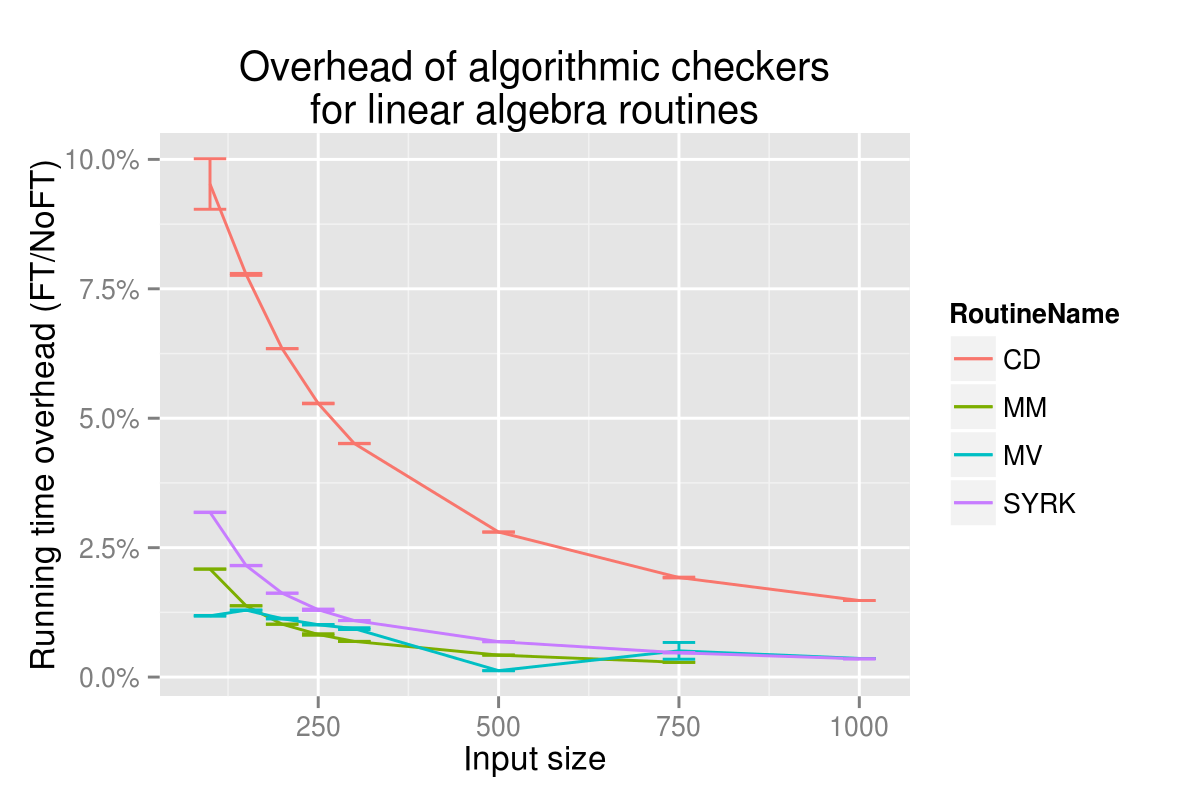
\includegraphics[width=1.00\columnwidth]{figs/4_1_1_Exp1_linalg}
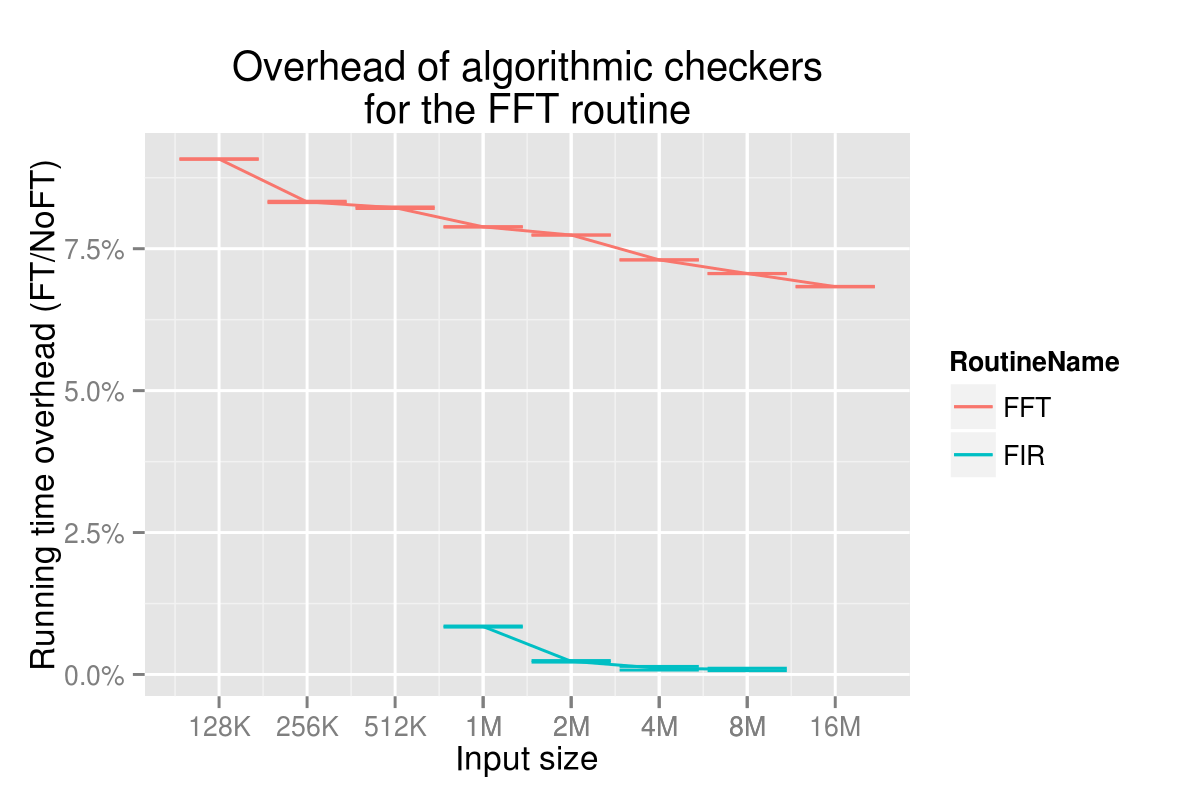
\includegraphics[width=1.00\columnwidth]{figs/4_1_1_Exp1_fft}
%\vspace{-5pt}
\caption{Overhead of resilience techniques when errors are not injected}
\label{fig:routine_detect_ovhd}
\end{figure}

%Experiment 1: Measure performance degradation of using error detectors as input sizes increase. In case of RK if we can run a version that doesn't do the multiple step sizes, do so but if this is difficult then don't worry about it.
We evaluate the costs of the above algorithmic error checkers by measuring their costs and effectiveness when running at different error rates on different types of inputs.
Figure \ref{fig:routine_detect_ovhd} measures the overheads of employing the algorithmic error detectors when no errors are injected, reporting the average of 100 runs.
The linear algebra routines were executed on $nxn$ square matrices where $n$ varies from 100 to 1000.
FFT ran on inputs vectors with 128K to 4M entries and RK ran on an integral with intervals $[0, t_1]$ where $t_1 \in \{10, 15, 20, 25, 30, 50, 75, 100\}$. The ODE system consists of a second-order nonlinear Van der Pol oscillator equation.
As our experiments show, the cost of algorithmic error detection is low and drops with increasing input sizes.

\begin{figure}[ht!]
%\vspace{-20pt}
\centering
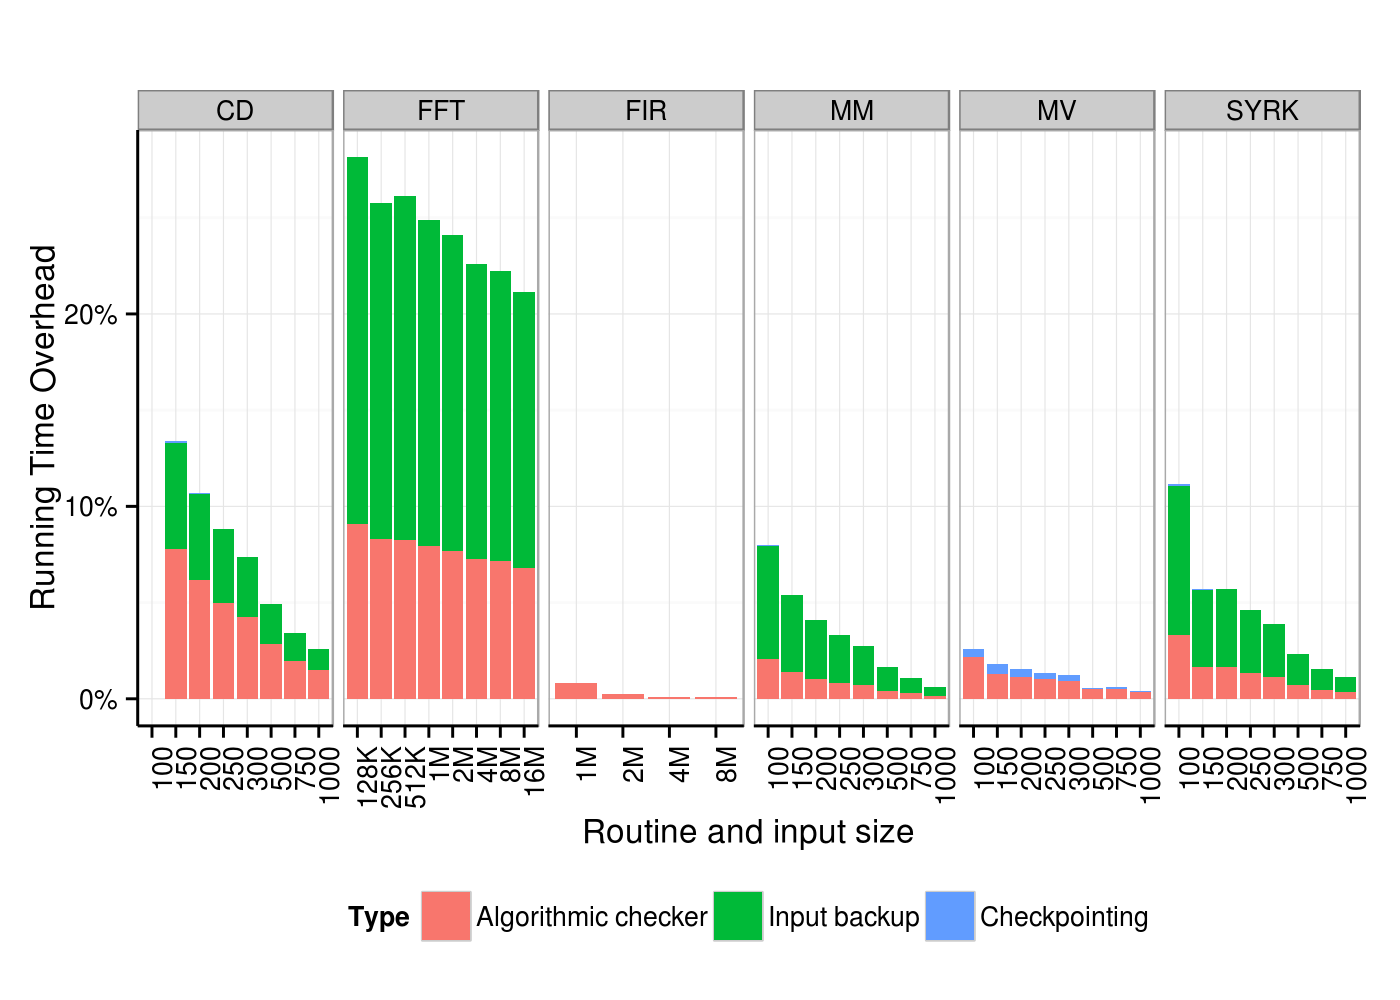
\includegraphics[width=1.00\columnwidth]{figs/4_1_1_Overall_Breakdown.png}
%\vspace{-5pt}
\caption{Overhead of resilience techniques. Results when no errors are injected are shown in the bars while overheads when errors are injected are expressed by using points.}
\label{fig:routine_all_ovhd}
\end{figure}

Figure~\ref{fig:routine_all_ovhd} shows in the bars the overhead of all resilience techniques with no fault injection.
The data shows that checkpointing routine's input (input backup bar) consumes more time than algorithm specific data corruption mechanisms (checker bar). In all cases, the overheads decrease as the input set size increses.
The same figure shows in the points the computational overhead when errors are injected. 
The data points within each figure are organized horizontally according to the average number of errors injected into runs with the given input size and at the given injection rate.
In general, those overheads also decrease when the input set size increases.  

%%%%%%%%%%%%%%%%%%%%%%%%%%%%%%%%%%%%%%%%%%%%%%%%%%%%%
\paragraph{Output Accuracy}
%\label{sec:res_tech:eval:accu}

\begin{figure}[ht!]
\centering
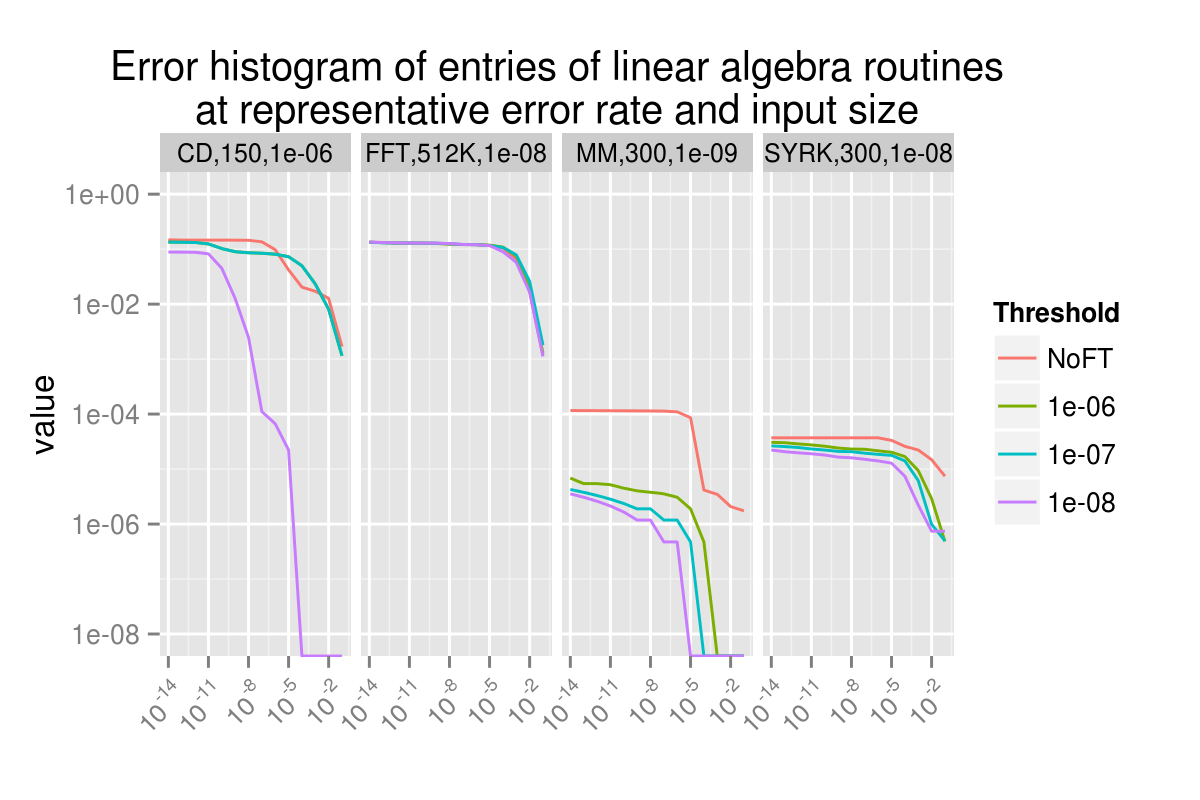
\includegraphics[width=1.00\columnwidth]{figs/4_1_1_Exp2_1_Example.png}
\caption{Error magnitude histogram showing the effectiveness of the error detector}
\label{fig:algo_err_dist}
\end{figure}

\begin{figure}[ht!]
\centering
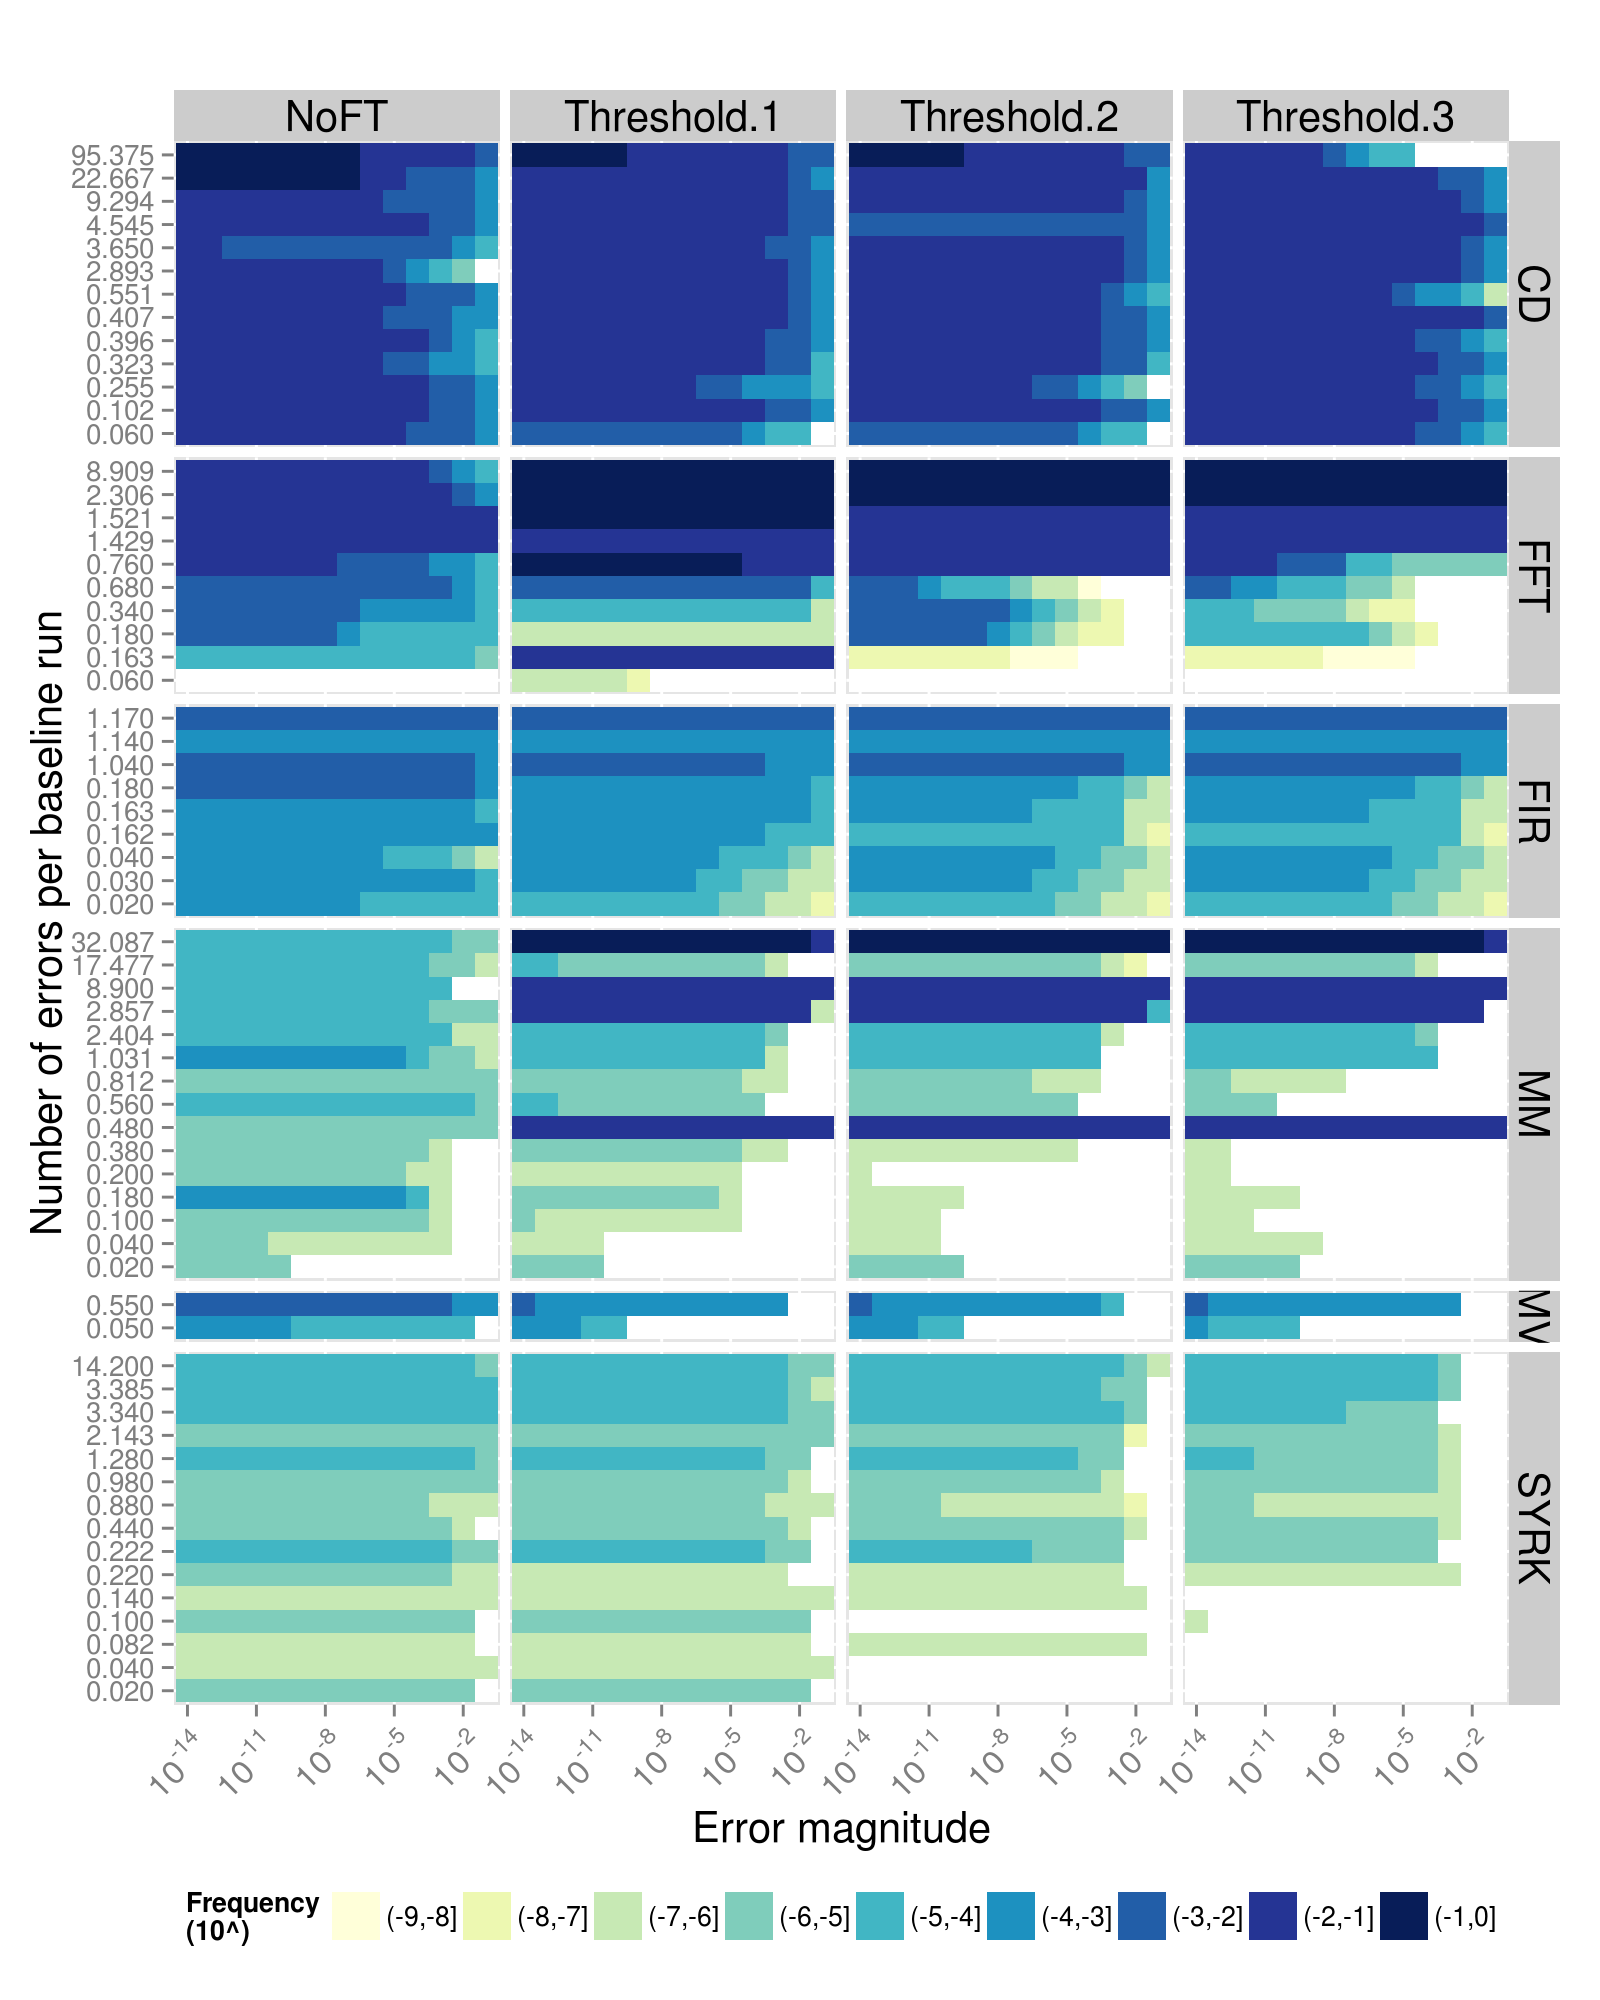
\includegraphics[width=1.00\columnwidth]{figs/4_1_1_Exp2_2_Heatmap_Error_ConfSpace.png}
\caption{Error magnitude histogram of the entire configuration space}
\label{fig:algo_err_heatmap}
\end{figure}

We now evaluate the effectiveness of our algorithmic detectors when errors are injected.
Figures~\ref{fig:algo_err_dist} show the fraction of entries in the outputs of each routine (y-axis) that have an error of a given magnitude (x-axis) as error magnitudes span from 1e-14 to 1e-4.
This figure is a focused view on few representative cases (each routine run on a single input size and error injection rate) across different resilience configurations: no error detection as well as detection thresholds of 1e-6, 1e-7 and 1e-8.
As the error magnitude increases the fraction of output entries with errors of that magnitude drops.
Importantly, the fraction of erroneous entries is reduced at all magnitudes as a result of error detection and restart.
Further, this reduction is more significant as the detection threshold shrinks since smaller magnitude errors are detected.

Figure~\ref{fig:algo_err_heatmap} shows the same information but for all experimental configurations: (i) input sizes of n=100 to 500 for linear algebra, 512K-8M size inputs for FFT and 10 100 for RK; (ii) error injection rates of 1e-7 to 1e-10.
The graph is a grid, with results for different routines listed vertically and different resilience configurations (no detection and different detection thresholds) listed horizontally.
The graph for each routine and resilience configuration presents the curves from Figure \ref{fig:algo_err_dist} as a heatmap.
The y-axis shows different routine input sizes and error injection rates, sorted according to the average number of error injections per run, in decreasing order from top to bottom.
The x-axis shows the different error magnitudes and the shade of each point is the fraction of the routine's entries that have a given error magnitude, with darker shades indicating more such entries.
Thus, each row of Figure~\ref{fig:algo_err_heatmap} represents the same information as each curve in Figure~\ref{fig:algo_err_dist}, with the shades of the squares representing the same information as the height of the line's points.

%We dont have the following figure and there is no time to generate it. 
%Figure~\ref{fig:algo_err_heatmap} shows the same information across the entire experimental space.
%The y-axis includes all algorithms, input sizes and error rates.
%The x-axis includes several segments for different degrees of error checking: none, as well as checking with thresholds \greg{???} \sui{1e-06, 1e-07 and 1e-08}. In each segment the x-axis spans over error magnitudes from \greg{???} \sui{1e-14} to \greg{???} \sui{1e-01}.
%The box associated with each combination of the four parameters the figure indicates the fraction of outputs that have an error of this magnitude by the shade of gray it is colored with, as indicated in the legend.
%The data shows that the accurate of application results is directly related to the number of errors that impact a given application run, rather than their rate.
%Further, it shows that a reduction of detection threshold is consistently effective at reducing the fraction of errors in each algorithm's output.
%However, the effectiveness of algorithmic checks has a limit, with CD and FFT showing moderate error vulnerability even at threshold 1e-8.
%\sui{(Rephrase) However, the algorithmic checkers cannot cover 100\% of the errors for CD, FFT and FIR, mainly fixing errors of large magnitudes which turned out to be effective in real applications (refer to the imperfect run rate plot for DRC.)}
%MM, MV and SYRK are significantly less vulnerable across the full range of error magnitudes.
%\sui{(Rephrase) The errors shown in MM, MV and SYRK are much more noticably fixed.}
%\greg{should reference vulnerability numbers more specifically}

%Experiment 3: Measure the fraction fraction of routine runs that are interrupted by the detection of an error.
%Display this information via the same heatmaps as above.

%\greg{For each experiment we need to include a discussion of what it means for how these checkers behave within the full-application runs.}

%\sui{The checkers have performed well in reducing erroneous results from the application outputs. Checkers for linear algebra are useful in removing errors from Lasso, as one could see from the results.}

%Those checkers can detect errors greater than a certain numeric threshold in those computations (determined by the user-defined error checker threshold). Once an error beyond the threshold has occurred, a re-calculation would be initiated.
%\greg{You need to be more specific. Each routine produces a result, your checker produces a result. How are these results compared and how is the threshold used to determine if there is an error or not.}

%In the following sections we would show that the error tolerance could not be arbitrarily small in order to be helpful in providing fault-tolerance when we take into account the checker itself may be unreliable since it's also vulnerable to soft errors.
%\greg{How is this shown? We certainly do show tighter detection tolerances cause longer executions, which cause more vulnerability. However, this is not the same as what you've just described}

%Although checkers are faster than the routines they protect, the unreliability of those checkers and the ensuing ``false alarms'' might trigger redundant re-calculations that are unnecessary, causing the application to run for much longer. This is specially true with an overly small error detection threshold. On the other hand, an overly loose detection threshold may fail to detect data corruption in output files. The results would be discussed in the results section.

\subsubsection{Runge-Kutta}
\label{sec:res_tech:eval:rk}

The difference between RK routine and others motivates special discussion of its resilience properties.
Since RK's adaptive step size mechanism is already effective at tolerating many numerical errors we used it as the error detector for this routine without adjusting its tolerance parameters.
The configurable portions of the RK resilience method are thus the choice of checkpointing and/or replication strategy.
Configurations \texttt{Ckpt} and \texttt{NoChkpt} denote whether checkpointing was used and configurations \texttt{Re} and \texttt{NoRe} denote whether replication was used.
We consider checkpointing periods equal to 1, $10^2$, $10^3$, $10^4$ and $10^5$ calls to the RK4 stepping function and the following replication configurations: No replication, 1 pair of replicas for each variable in the source code and 1 pair of replicas for each occurrance of each variable in the source code.

\paragraph{Overheads}
%\label{sec:res_tech:eval:ovhd}

%\begin{figure}[ht!]
%%\vspace{-20pt}
%\centering
%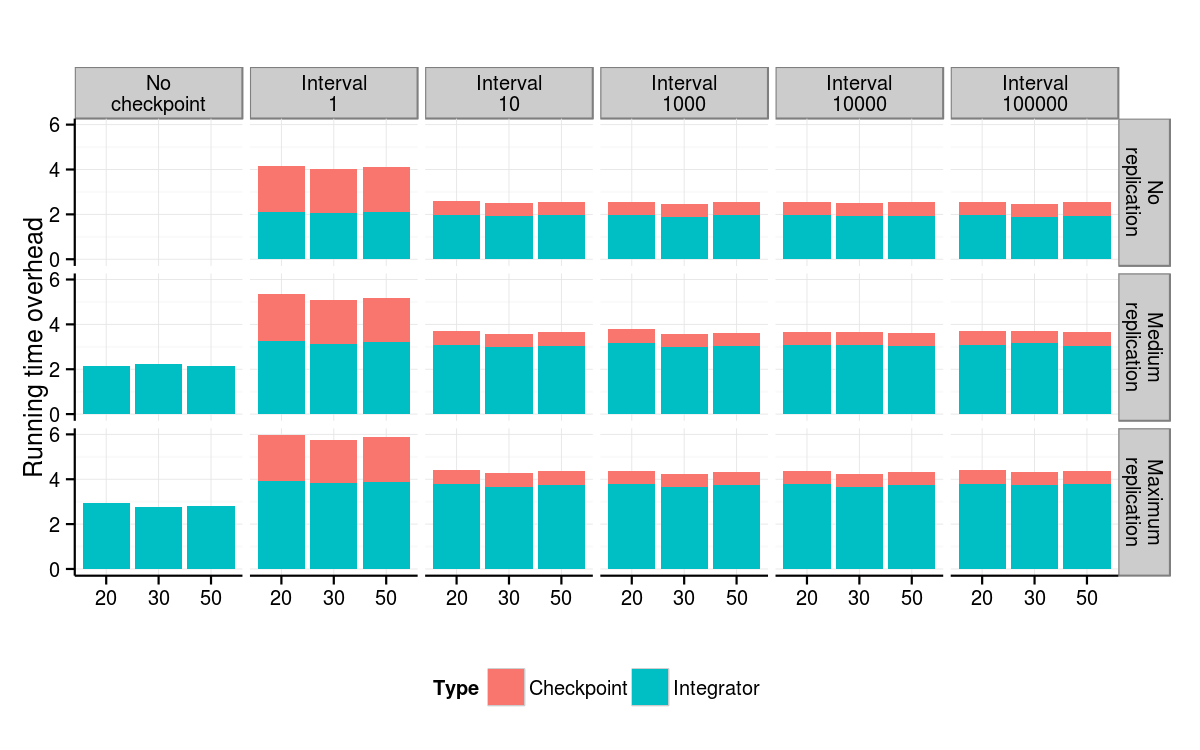
\includegraphics[width=1.00\columnwidth]{figs/4_1_1_Overall_Breakdown_RK4}
%%\vspace{-5pt}
%\caption{Overhead of resilience techniques for RK when errors are not injected}
%\label{fig:rk_routine_detect_ovhd}
%\end{figure}

%Figure~\ref{fig:rk_routine_detect_ovhd} shows the overhead of employing each of the four RK resilience techniques when no errors are injected. We use here the same format as in figure\ref{fig:routine_all_ovhd}. 
%%MARC: I decided to remove the above figure because it doesnt make sense to me and the same information is displayed in the following figure with more readibility.

\begin{figure}[ht!]
\centering
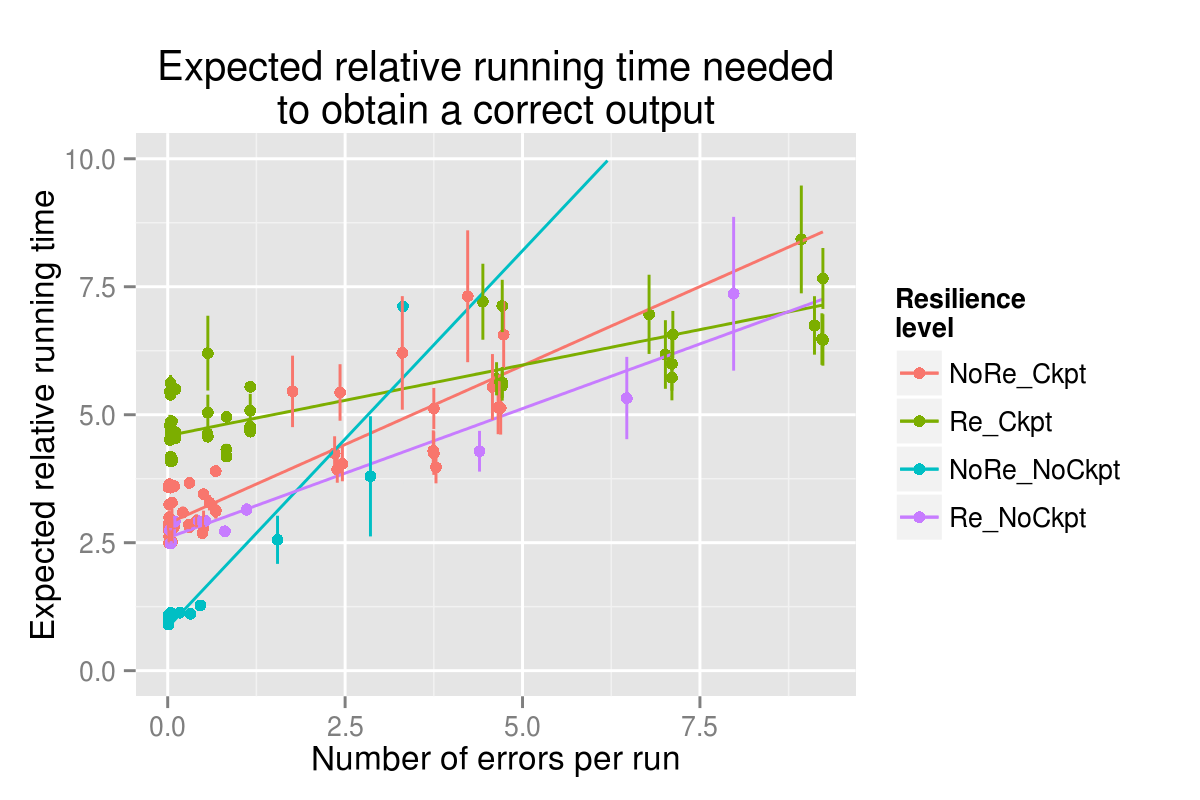
\includegraphics[width=1.00\columnwidth]{figs/4_1_2_Exp2_Expected_Running_Time_Needed.png}
\caption{Overhead of resilience techniques for RK when errors are injected}
\label{fig:rk_routine_exp_exec}
\end{figure}

Figure~\ref{fig:rk_routine_exp_exec} shows the RK's overhead when 0 up to 10 errors per run are injected.%, using the same format as Figure~\ref{fig:routine_exp_exec}.
Although the \texttt{NoRe\_NoCkpt} configuration has the lowest overhead when only a few errors are injected (low error rate or small execution times), as the number of errors per run increase this configuration quickly becomes extremely slow because an error is detected in almost every run.
Since each such detection requires a restart of the routine, at higher error rates this causes RK to restart many times before it completes.
In contrast, while the other configurations have a higher overhead for a few errors per run, their execution time scales much better with increasing error rates, making them significantly more practical.
By varying the checkpointing interval and the degree to which various RK variables are replicated it is possible to achieve a wide range of design points that provide the best performance at various error rates.

\paragraph{Output Accuracy}
%\label{sec:res_tech:eval:accu}

\begin{figure}[ht!]
\centering
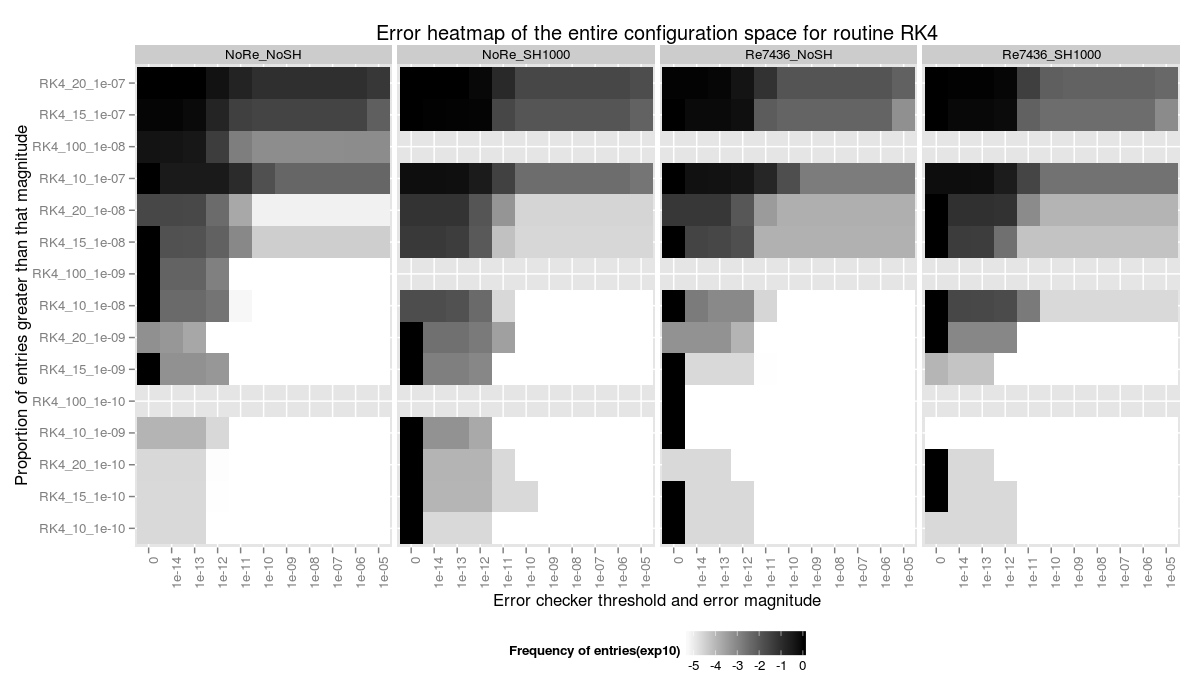
\includegraphics[width=1.00\columnwidth]{figs/4_1_1_Exp2_2_Heatmap_Error_ConfSpace_RK4.png}
\caption{Error magnitude histogram of the entire configuration space of RK}
\label{fig:rt_algo_err_heatmap}
\end{figure}

\begin{figure}[ht!]
\centering
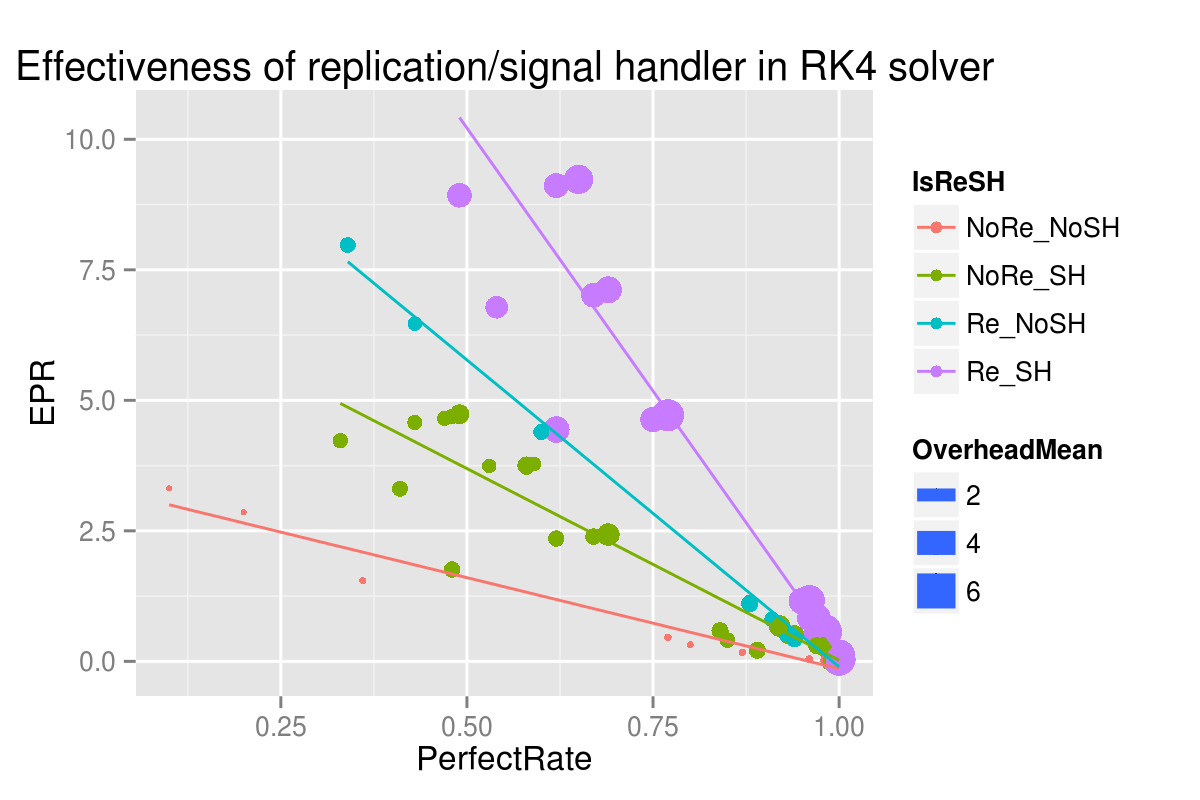
\includegraphics[width=1.00\columnwidth]{figs/4_1_2_Exp2_Effectiveness.png}
\caption{Fraction of RK runs that achieve low error (smaller than 1e-7).}
\label{fig:rk_effectiveness}
\end{figure}

Figure~\ref{fig:rt_algo_err_heatmap} shows the fraction of errors in RK's outputs for the four resilience configurations, in the same format as Figure~\ref{fig:algo_err_heatmap}.
It shows that the use of either resilience approaches significantly reduces RK's vulnerability to soft errors and the use of both techniques is even more effective.
Figure~\ref{fig:rk_effectiveness} shows this from a different perspective: the fraction of RK runs where the root-mean-squared error of the output vector is below 1e-7 (y-axis), relative to the number of error injections per run (x-axis).
It shows that RK configurations with higher level of resilience are able to achieve this accuracy target more frequently.
This is primarily because by avoiding frequent rollbacks due to crashes these techniques reduce the total number of errors that are injected into the application run, which also reduces the probability that one such error will be missed by RK's algorithmic error detector.
As with overhead, the choice of checkpointing interval and replication degree make it possible to choose a wide range accuracy levels and probabilities that these targets will be satisfied.

%
%???\sui{the effectiveness of the error handlers and the error checkers. Note that the graph shows fault injection experiments at various rates (defined by errors per run).}
%
%\sui{There are roughly three types of fault rates: 1) very high fault rates (more than tens of errors per run), under which the application would barely complete running; 2) medium fault rates (1 to 10 errors per run), where the rate that the application completes running is very sensitive to the fault rate (because for a non-resilient application, just one error is enough to cause a segmentation fault and abort the application) and 3) low error rates, smaller than 1 errors per run. The effectiveness of the fault detector is most visible at fault rates from under 1 faults per run to several errors per run, which is visible from the histograms that the vertical bars indicating a run with algorithmic detectors is generally brighter, therefore less erroneous; when the error rates goes beyond 10 errors per run, the effectiveness of the signal handlers become more noticeable, rising the chance the application would complete.}
%
%\sui{At higher error rates, the signal handlers enable more runs to complete as well as allowing erroneous results to go into the output. More erroneous results are allowed into the final output by the signal handler than the erroneous intermediate corrected by the algorithmic checker. That is why from the histograms, some vertical bars indicating fault-tolerant runs at a very high error rate would look darker.}
%
%
%
%
%
%
%Errors that do not cause the application to access an invalid memory location are detected by replicating key pointers and loop iteration variables.
%The Hattrick application uses a high-accuracy ODE solver that is capable of estimating errors and detecting and reducing errors to a certain level adaptively.
%Therefore we would only focus on the application's vulnerability to pointer and index corruptions.
%Replicating critical variables (pointers and indices) and leveraging Byzantine fault tolerance and correcting those pointers and indices during run-time would raise the applications' resistance to soft errors \sui{and increase the chance this application would output correct results.}
%
%\sui{Unlike the numerical and FFT routines used in the other two applications, the ODE solver has an stepping function called on the evaluation(s) of each integration step (GSL performs two evaluations per timestep in order to estimate integration error and perform adaptive step size control), which is called much more frequently, on the magnitude of millions of times during the lifetime of the application. Contrarily, the linear algebra routines are only called less than a hundred times during the execution of Lasso with a 10x input, and the FFT routines are called only several hundred times during the execution of DRC with a 30x input. Both are moderate-sized inputs in our experiments.}
%
%\greg{Need to explain why we only do this for Hattrick.} \sui{The checkpointing scheme used here has overhead of having to set signal handlers and perform up-to-date checksum computation of critical data structures. The more often the routines are called, the more frequent the critical data structures need be kept up-to-date, therefore this overhead is larger (non-trivial compated to that for FFT and linear algebra) for a frequently called routine like the integrator. This overhead makes the fault tolerance technique less efficient as it was in linear algebra and FFT routines, bringing it to the same ballpark as the expensive pointer replciation technique. Although it is possible to reduce the frequency of updating the checkpoints, it would also reduce the effectiveness of this method sharply.}
%
%\sui{
%The other reason is, pointer replication performs a better job at maintaining the chance the routine generates correct results (See figure \ref{fig:rk4_eff_ovhd}). As mentioned before, the RK4 integrator does not have an effective checker that takes its output and tells the user whether the output is correct. As the user can't know whether a re-run is necessary and the user should be concerned by the expected time by which s/he can expect a correct output. Therefore, a higher chance of producing correct results would lower the expected cost the user would have to pay to get the correct result despite the overhead. The method of computing this expected running time is described in greater detail in section \ref{sec:eval:perf}'s Markov Model. From \ref{fig:rk4_eff_ovhd} one could see the ratio of perfect runs out of all runs (that are completed or incomplete) and the number of faults per run forms an almost linear relationship. The linear regression model is used to evaluate the position of the guide points needed for the following experiments.
%}
%
%\sui{Refer to Figure \ref{fig:rk4_eff_ovhd} one could see the number of expected running time of different configurations if one wants to get a correct output from the application in a faulty environments. As the number of faults injected per run increases, the expected running time of the original, non-fault-tolerant application increases at a much faster rate than the other fault-tolerant counterparts. In real life scientific applications that run much longer, it's likely that a fault could hit the application several times before it completes. In such situations, the replication-only resilience technology produces the least expected number of runs needed to get a correct answer.}
%
%To determine a replication strategy we have to determine which variables to replicate and how many replicas to use for replicating them. The following two subsections would be focused on these problems.
%\greg{The report spends a lot of space talking about this but in the end the conclusion is that we just a pick a few options and evaluate them experimentally. How much space should we devote to this discussion.}
%
%Experiment 2: Measure the effectiveness and performance costs of replication. Need to explain why we don't use it for Lasso and DRC.
\section{Evaluation of Resilience Methodology in Applications}
\label{sec:eval}

Having evaluated the resilience properties of the individual application routines and resilience techniques we now consider our three target applications ADDR, Hattrick and DRC.
Section~\ref{sec:eval:perf} reports on the impact of errors and resilience techniques on application performance. Section~\ref{sec:eval:acc} describes the distribution of errors in the results of these applications.
These results are based on a fault injection campaign that includes a range of fault injection rates, input sizes and configurations of resilience mechanisms, with 100 application runs for each combination of parameters.
This corresponds to a total of 66100 for lasso, 43200 for DRC, 102000 for Hattrick error injection experiments.

A given application run may terminate successfully or crash due to an unrecoverable error.
Unrecoverable errors occur when there is a segmentation fault in code outside our protected routines or if 5 rollbacks of a routine have been observed in a given run since such repeated rollbacks almost always indicate that the corruption in application state cannot be repaired.
Since we assume that the user needs application results regardless of the error rate, if the application crashes it is restarted from the beginning as many times as needed for it to complete.

To evaluate the behavior of these applications in a broad range of error environments we consider several error injection rates.
For reference, assuming a typical FIT of 100-100,000 for individual processing cores (FIT = failure in one billion hours of operation and this range has been experimentally observed for commodity electronics~\cite{mem_errors:2010}), an HPC system with one million cores will experience .1-100 errors per hour, which is equivalent to 3e-11 - 3e-14 errors per processor cycle on a 1Ghz processor.
The range of error injection rates used used in our experiments were chosen such that (i) on average one or more errors were injected in the executions of our target applications and (ii) at least some application runs completed without crashing.
Results for error rates that induce fewer than one error per run were extrapolated from our experiments with higher error rates.
This was done by considering only the runs where exactly one error was injected and trivially scaling the results to correspond to 1 in every $n$ runs being injected with an error while remaining $n-1$ runs complete with no injection.

%\greg{This is the section where we put all the pieces together and present the experimental results on full applications. We should describe our main use-case here: user wants to achieve a given accuracy with a given probability and we configure the algorithm to provide this at the lowest cost. QUESTION: how do we pick the parameters of each resilience technique? Which metric is being optimized?} \sui{Using the choices of those parameters derived from the experiments we have already performed (treat it as a ``training set'') and use those choices on some new experiment configurations (treat as ``test set''), and see what is the probability that those choices could satisfy the users' experiments.}

\subsection{Performance Impact}
\label{sec:eval:perf}

Our fault injection experiments ran each application configuration to completion, recording whether it completed and if so, the magnitude of the error.
We calculate the execution time of each configuration, accounting for application rollbacks via the formula $\frac{t_c}{1-p_f}$, $t_c$ is the average completion time of such runs and $p_f$ is the probability of a run failing to complete.
Figures~\ref{fig:Lasso_EstdCost}, \ref{fig:DRC_EstdCost} and \ref{fig:Hattrick_EstdCost} show the expected execution time, relative to the execution time of the non-fault tolerant version of the application when no errors are injected, of the non-fault tolerant version (red) and the optimal fault tolerant version (blue). 
The optimal fault tolerant version is the one that suffers from smaller overhead among the ones that provide more resilience enhancement. 
To select the optimal one we consider error checker tresholds from $10^{-4}$ to $10^{-7}$ for ADDR, from $10^{-6}$ to $3 \cdot 10^{-8}$ for DRC and from using one pair of copies for each variable occurence to using a different pair of replicas for each variable occurrence for Hattrick.     
The graphs from left to right correspond to different application input sizes.
Within each graph the x-axis corresponds to error injection rates, while the y-axis shows the relative execution time, both logarithmic.

For each configuration we plot a 95\% confidence interval.
This is the range of relative execution times at the given error rate and application configuration in that will occur in 95\% of all trials.
The confidence interval is computed by modeling the number of times application results will meet the error bound using a Binomial distribution.
Given a binary random variable that is equal to 1 (i.e. error bound achieved) with probability $p$ and 0 (i.e. bound missed) with probability $1-p$ the Binomial distribution is the number of trials where it is 1.

Figure~\ref{fig:Lasso_EstdCost} shows that the non-fault tolerant ADDR slows down from 2x to 9x, depending on the input set size, as a result of the injected faults.
The optimal fault tolerance version the algorithm shows degradation that are around one half of the non-faul tolerant one, which implies that our technique improve ADDR's resilience by 50\%. 

Figure~\ref{fig:DRC_EstdCost} shows results regarding the DRC application. 
Since it performs many more integer operations and memory copies than ADDR, it is more vulnerable to errors that corrupt the values of pointers or cause loads and stores to target invalid memory locations.
Such errors cause memory segmentation faults, which force DRC to restart its execution and thus incur a very high overhead. 
That is the reason why the performance slowdown of its non-fault tolerant version is much larger than the ADDR one. 
In contrast, the optimal fault tolerant version reduces almost completely the slowdown due to fault injection.   

Figure~\ref{fig:Hattrick_EstdCost} shows how the performance slowdown of the fault tolerance version it is very unstable but it can reach values close to 100x. 
The performance of the optimal fault tolerant version is consistently much better.     

\begin{figure*}[ht!]
\centering
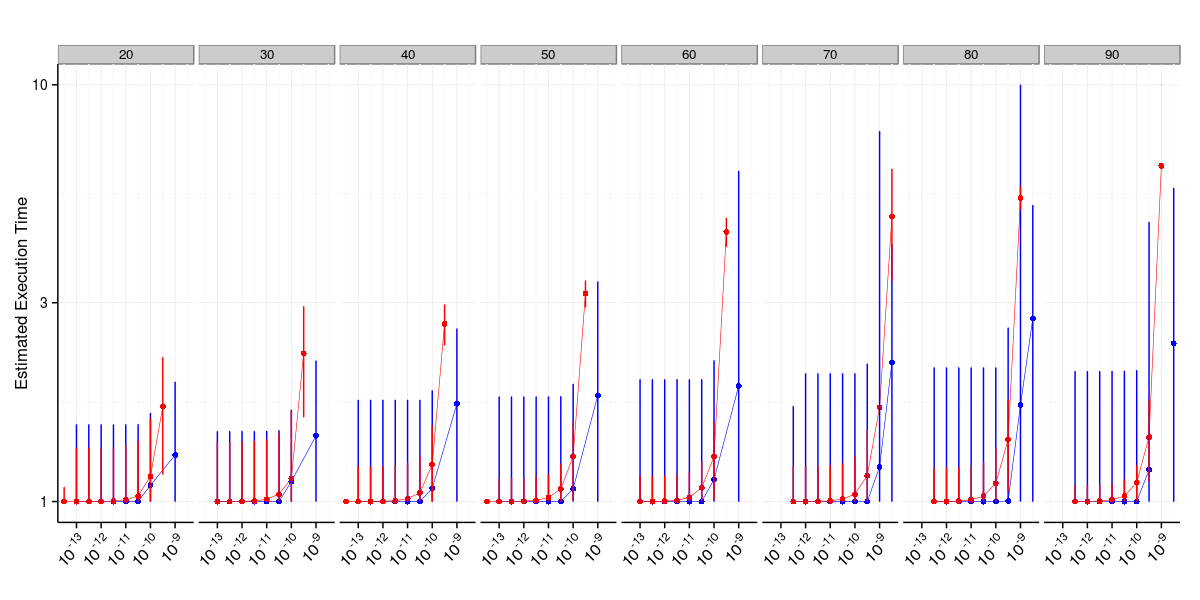
\includegraphics[width=2.00\columnwidth]{figs/Lasso_EstdCost.png}
\vspace{-10pt}
\caption{Execution time of ADDR relative to non-fault tolerant fault-free execution time. Results for the non-fault tolerant version (red) and the optimal fault tolerant version (blue) are shown.}
\vspace{-10pt}
\label{fig:Lasso_EstdCost}
\end{figure*}

\begin{figure*}[ht!]
\centering
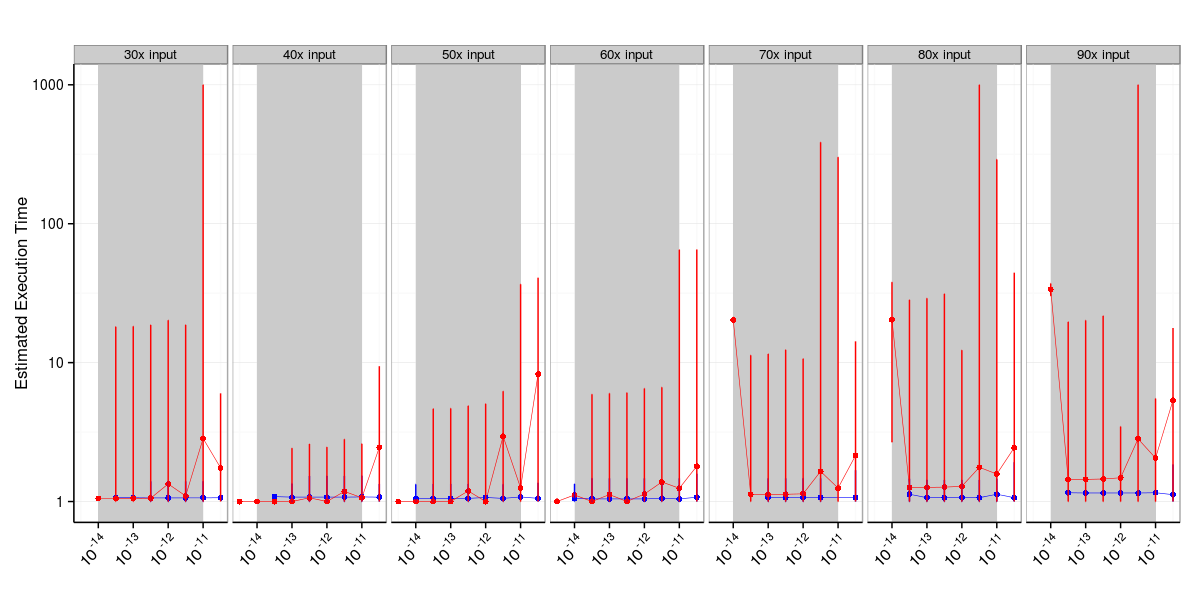
\includegraphics[width=2.00\columnwidth]{figs/DRC_EstdCost.png}
\vspace{-10pt}
\caption{Execution time of DRC relative to non-fault tolerant fault-free execution time. Results for the non-fault tolerant version (red) and the optimal fault tolerant version (blue) are shown.}
\vspace{-10pt}
\label{fig:DRC_EstdCost}
\end{figure*}

\begin{figure*}[ht!]
\centering
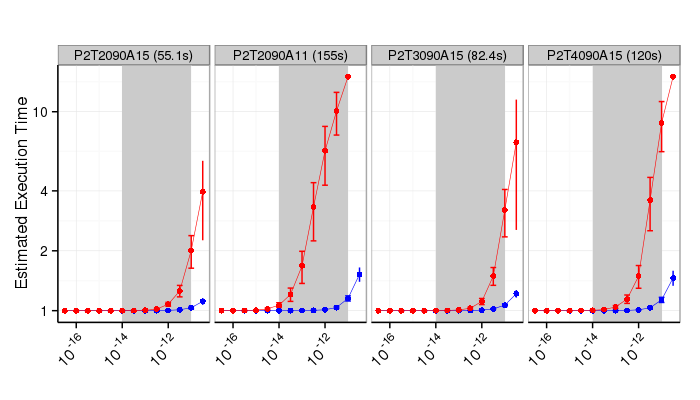
\includegraphics[width=2.00\columnwidth]{figs/Hattrick_EstdCost.png}
\vspace{-10pt}
\caption{Execution time of Hattrick relative to non-fault tolerant fault-free execution time. Results for the non-fault tolerant version (red) and the optimal fault tolerant version (blue) are shown.}
\vspace{-10pt}
\label{fig:Hattrick_EstdCost}
\end{figure*}


%\sui{When a user wants to run an application under a faulty environment and obtain correct results, s/he would have to expect to run a part of this application multiple times in case the application aborts due to memory access errors or return useless incorrect results. The user might want to have the application return to a certain checkpoint, or restart the entire application should any unrecoverable occurs. The cost of rollback, and the chance of each type of errors occurs at a different rate. The Markov model comes into play here with its capability to capture all these parameters of experiments we have already run and predict the running time of the applications at configurations not experimented with.}


%Experiment 1: Measure the slowdown of each application at the optimal configuration
%Experiment 2: Measure the rate of aborts due to algorithmic errors, segfaults and redundant copy mismatches (separate the causes)

\subsection{Result Accuracy}
\label{sec:eval:acc}

%Experiment: Measure the accuracy of the results produced in completed runs, including error bars on the variability of the errors

If the probability that a given run completes without an unrecoverable error is greater than 0 then the application will eventually complete with some output after some number of restarts.
This section evaluates the distribution of errors in the resulting outputs.
The outputs of the different applications are as follows:
\begin{itemize}
    \item ADDR: vector that holds the solution to the linear system.
    \item Hattrick: vector that holds the state of the n-body system at the final application time-step, with 6 numbers per body.
    \item DRC: a Pulse Code Modulation-formatted file, which is a sequence of numbers.
\end{itemize}
Since the outputs of each routine can be represented as vectors we calculate the error in the outputs by comparing the vector $v_e$ returned by each routine when errors are injected to the correct vector $v_c$ computed during a fault-free run and computing the L2 norm of the difference: $\sqrt{\frac{\sum_{i} (v_c-v_e)^2}{\left| v_c \right|}}$.

Figures~\ref{fig:Lasso_ImperfectRate}, \ref{fig:DRC_ImperfectRate} and \ref{fig:Hattrick_ImperfectRate} show the errors in application results from a user-centric perspective.
Given a user-specified error magnitude that must be satisfied by application results these figures plot the fraction of application runs for which this target was satisfied
From left to right each figure shows graphs for different input sizes and from top to bottom it shows results for different error magnitude bounds.
The x-axis in each graph shows the fault injection rate (logarithmic) while the y-axis shows the fraction of runs where the error target was satisfied (linear).
Each graph shows data for the non-fault tolerant version of the application (all points connected by the line) as well as all the the fault tolerant versions (optimal configurations connected by a line).
The 95\% confidence interval is plotted and denoted range of probabilities that the error bound will be achieved at the given error rate and application configuration in 95\% of all trials.

\greg{Sui, please confirm that the following is true} \sui{Yes. ADDR is sensitive to errors, and even a small number of error would cause noticable errors in the results. Comparing the leftmost data points on the ``probability of not satisfying'' graphs of the 3 applications.}
The data shows that the probability that the non-fault tolerant version of ADDR satisfies the user-provided error bound is low, for bounds randing from 1e-10 to 1e-4.
In contrast, the fault tolerant version of the application is significantly more successful, especially for error rates of 1e-12 and lower (\greg{need log plot to show the low accuracy rate more precisely} \sui{Changed to log plot.}).
\greg{Can mention the fact that the fault tolerant versions are most successful for loose error bounds and small inputs but the success rate is poor for the 10x input. Why?} \sui{I know why. After inspecting Lasso's code, it turns out Lasso contains TWO branches of code: one on ``fat'' matrices and the other on ``skinny'' matrices. Only 10x input triggers the ``fat matrix'' code and inputs 20 through 100 would trigger the ``skinny'' code. The two versions of code are not the same therefore they would be vulnerable to soft errors to different degrees.}

\greg{I won't comment on the DRC errors because Sui is currently trying to improve them. Right now we're not being very successful. However, since DRC is a single precision code, we should really be considering much larger error bounds, like 1e-6 or 1e-4}. \sui{Expanding the ranges makes sense. Plus, I think the range for Hattrick can be as tight as 1e-20. I have used 1e-17, 1e-14 and 1e-10 in the updated visualization.}

\greg{Its hard to comment on Hattrick until we have a version of the plots with a logscale y-axis since it'll tell us exactly how successful the fault tolerant versions of the code are. Also, what are the relative execution times of these input files? This will give us an idea of how vulnerable they are.} \sui{Input 1=55s; Input 2=155s; Input 3=82s; Input 4=120s }

\begin{figure*}[ht!]
\centering
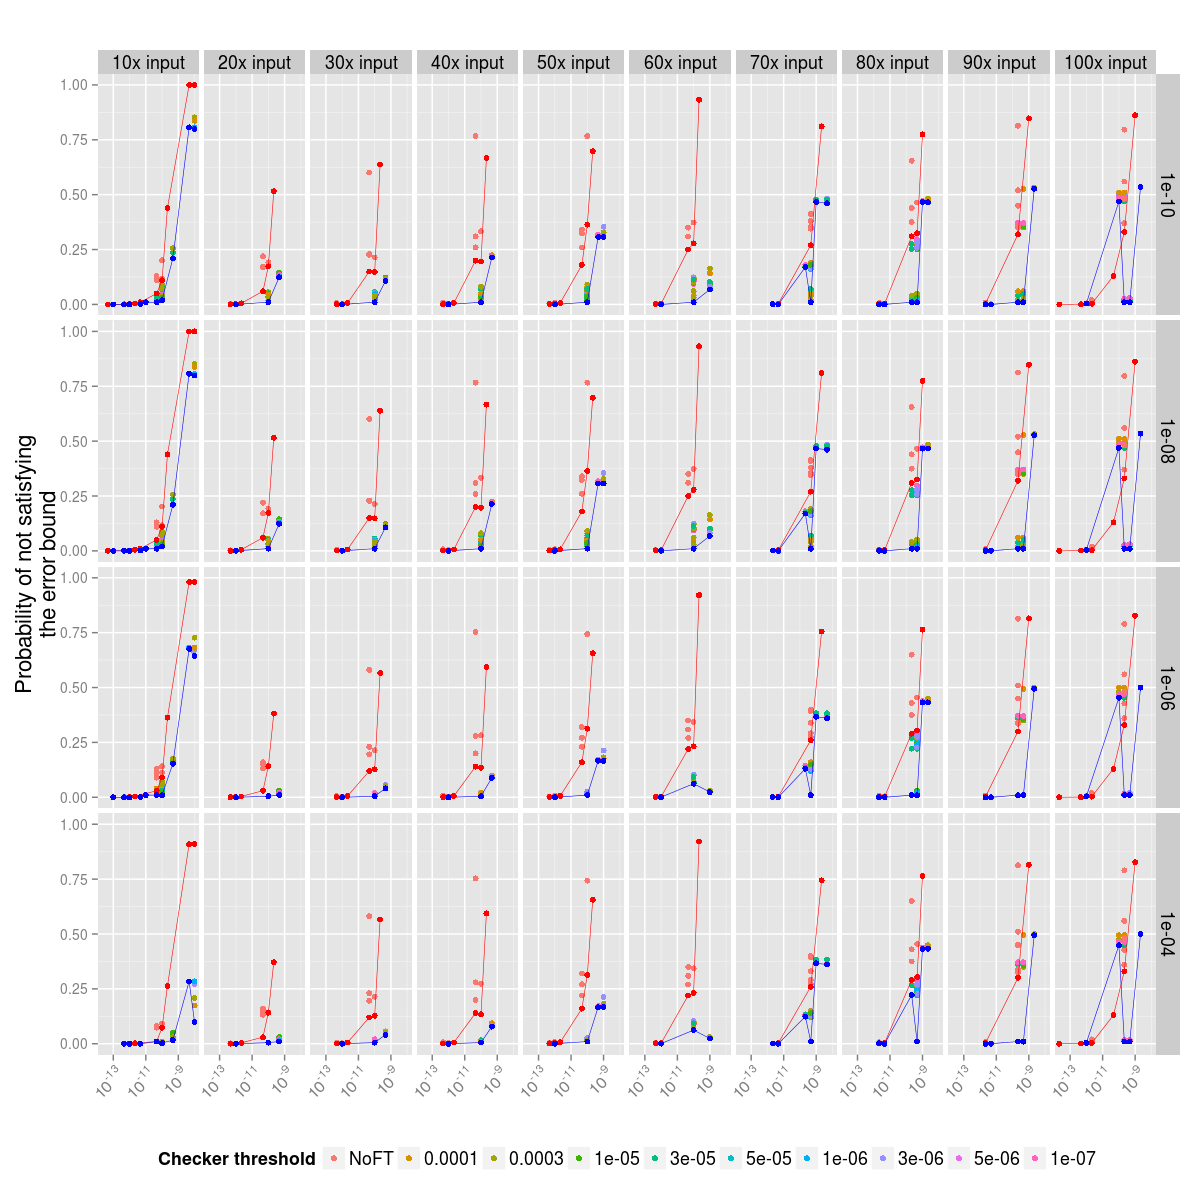
\includegraphics[height=5in]{figs/Lasso_ImperfectRate.png}
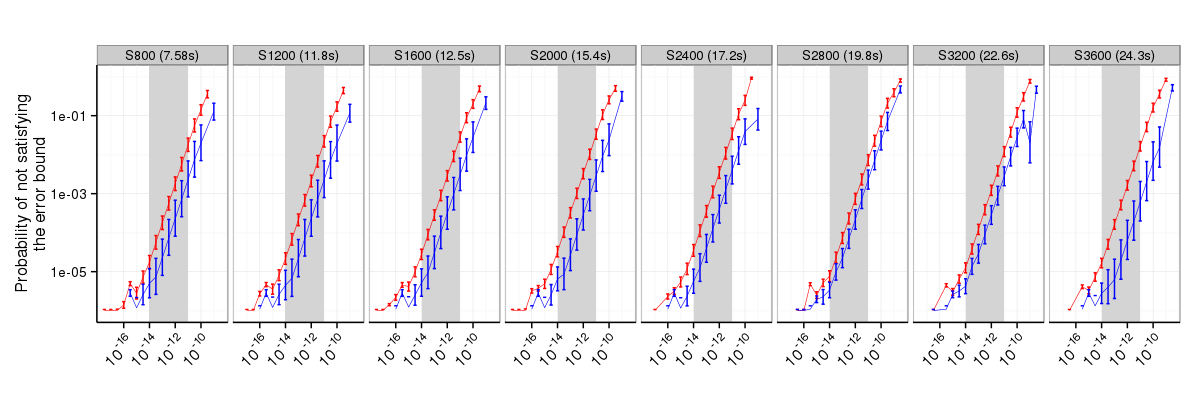
\includegraphics[height=5in]{figs/Lasso_ImperfectRate_log.png}
\caption{Probability of not satisfying the user-provided error bound for ADDR \greg{why do the probabilities of the no-FT version not change as the error threshold changes? Also, it may be good to show fewer columns but add graphs where the y-scale is a log-plot} \sui{Added a log plot.}}
\label{fig:Lasso_ImperfectRate}
\end{figure*}

\begin{figure*}[ht!]
\centering
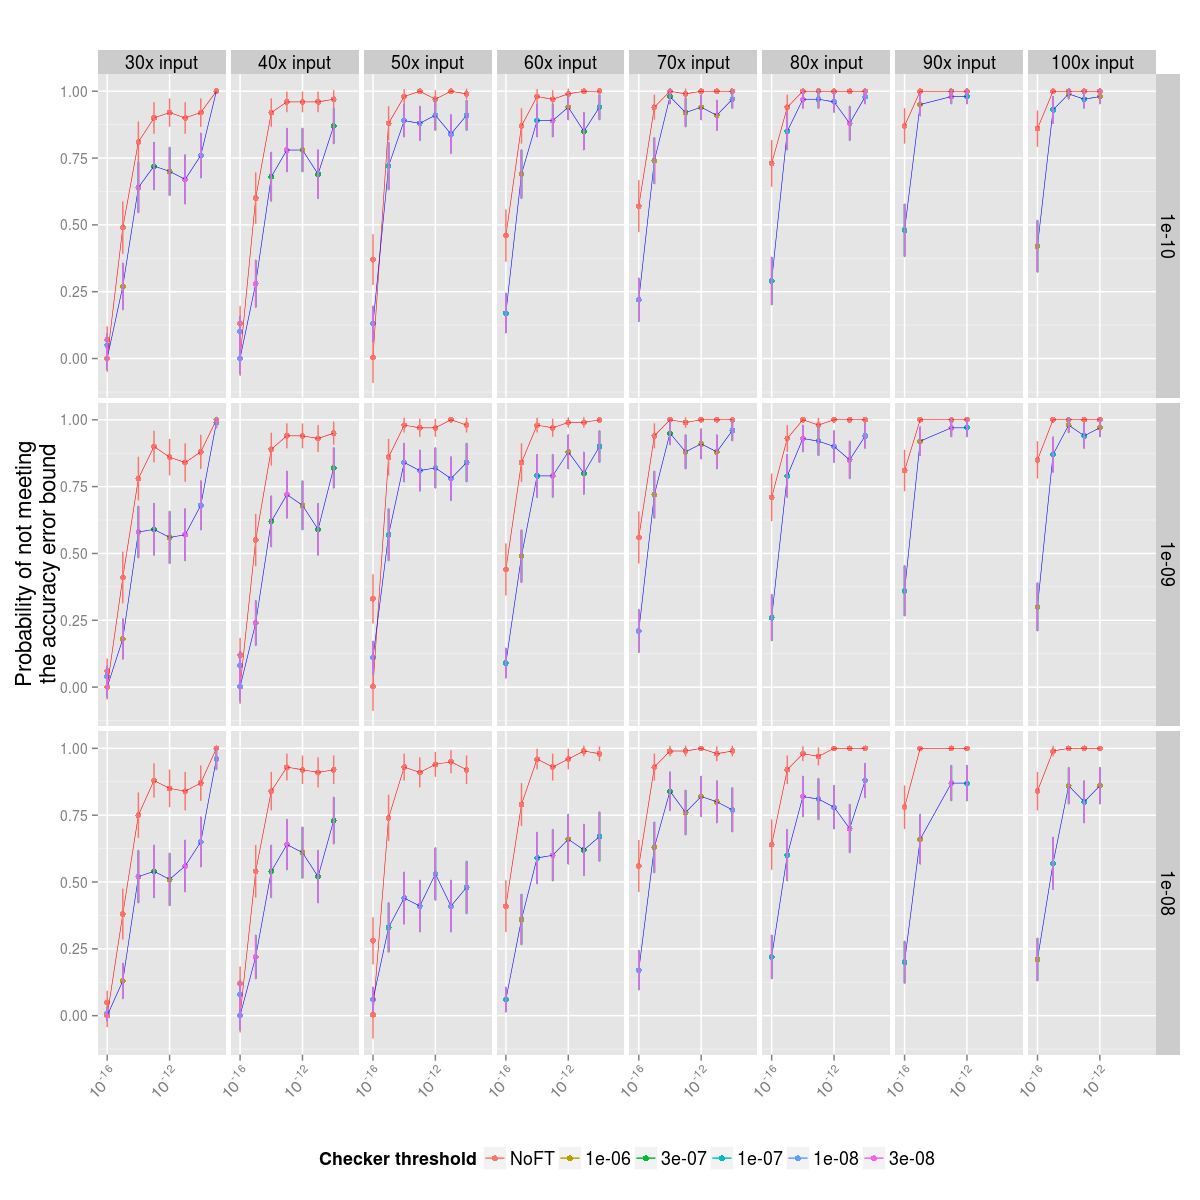
\includegraphics[height=3in]{figs/DRC_ImperfectRate.png}
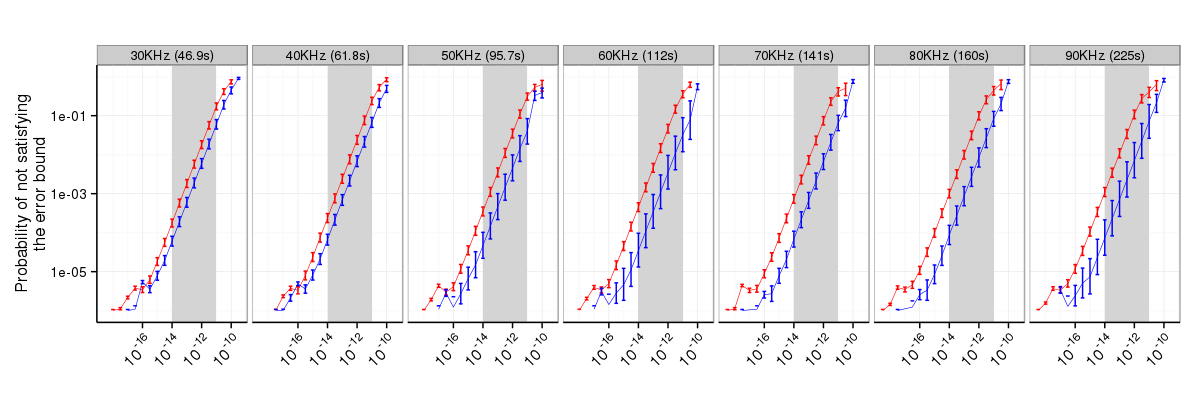
\includegraphics[height=3in]{figs/DRC_ImperfectRate_log.png}
\caption{Probability of not satisfying the user-provided error bound for DRC \greg{why do the probabilities of the no-FT version not change as the error threshold changes? Also, it may be good to show fewer columns but add graphs where the y-scale is a log-plot} \sui{Added a log plot (on the right).}}
\label{fig:DRC_ImperfectRate}
\end{figure*}

\begin{figure*}[ht!]
\centering
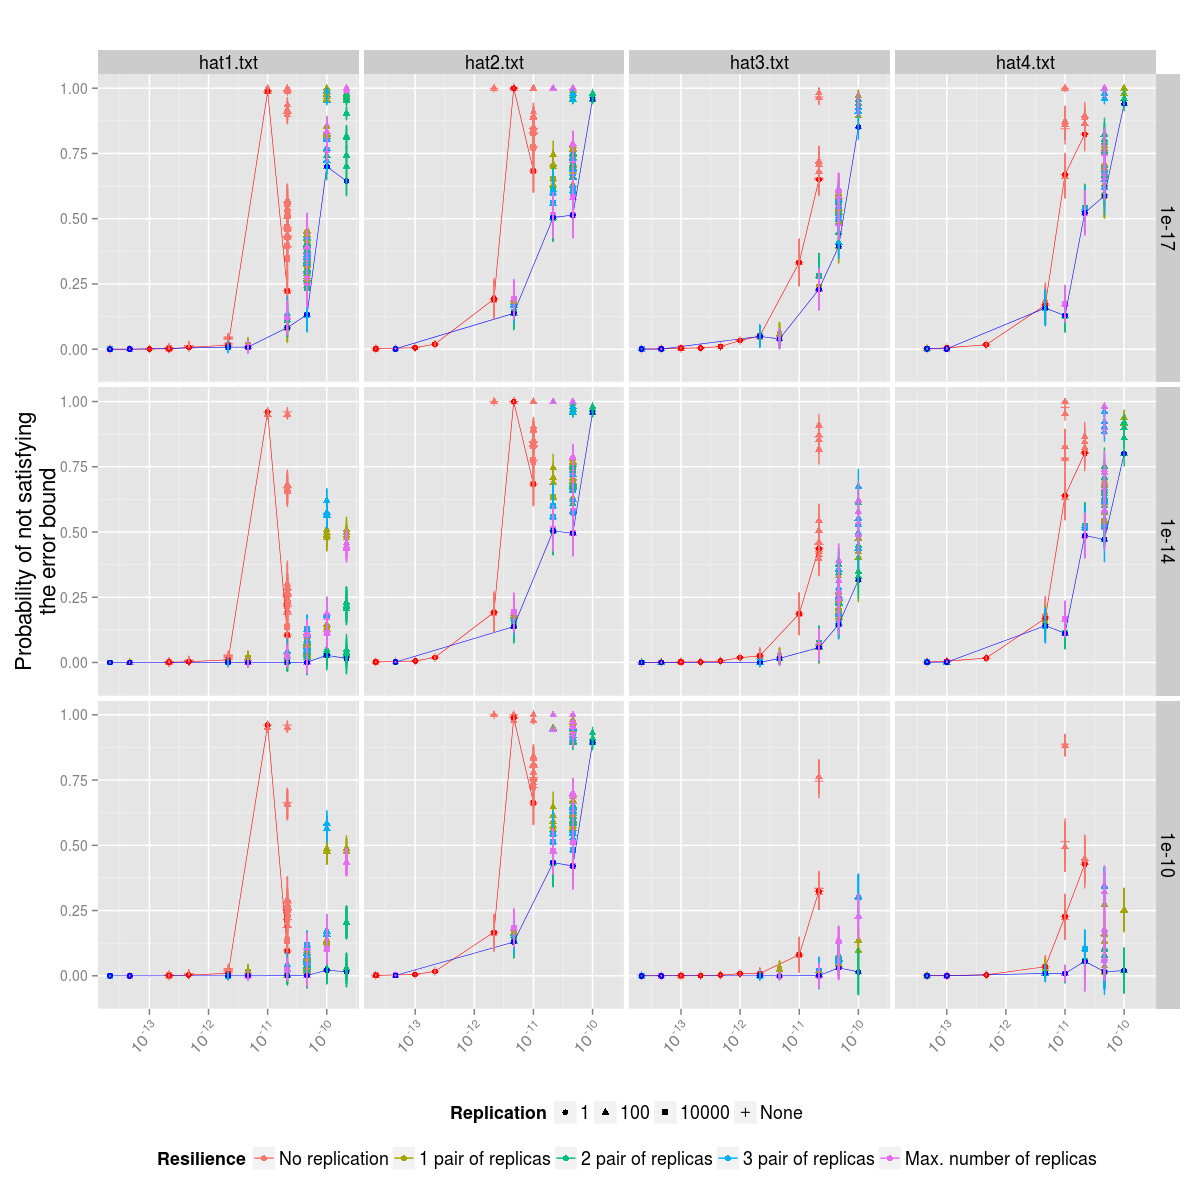
\includegraphics[height=3in]{figs/Hattrick_ImperfectRate.png}
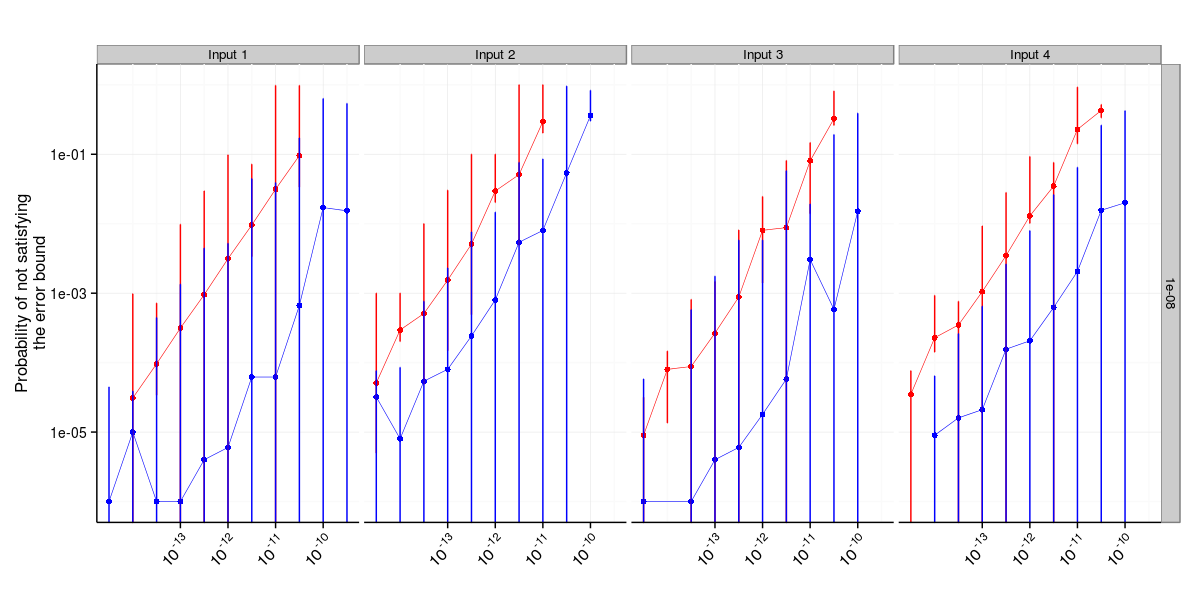
\includegraphics[height=3in]{figs/Hattrick_ImperfectRate_log.png}
\caption{Probability of not satisfying the user-provided error bound for Hattrick \greg{why do the probabilities of the no-FT version not change as the error threshold changes? Also, it may be good to show fewer columns but add graphs where the y-scale is a log-plot} \sui{The change is small therefore not visible on a linear scale. Switching to log plot revealed those tiny differences.}}
\label{fig:Hattrick_ImperfectRate}
\end{figure*}

\subsection{Overall Evaluation}
\label{sec:eval:overall}

%Experiment: Final graph that shows slowdown for each desired probability of perfect results.

\section{Summary}
\label{sec:summary}

\bibliographystyle{abbrv}
\bibliography{bibs}

\end{document}
